\begin{figure}[H]
\centering{}
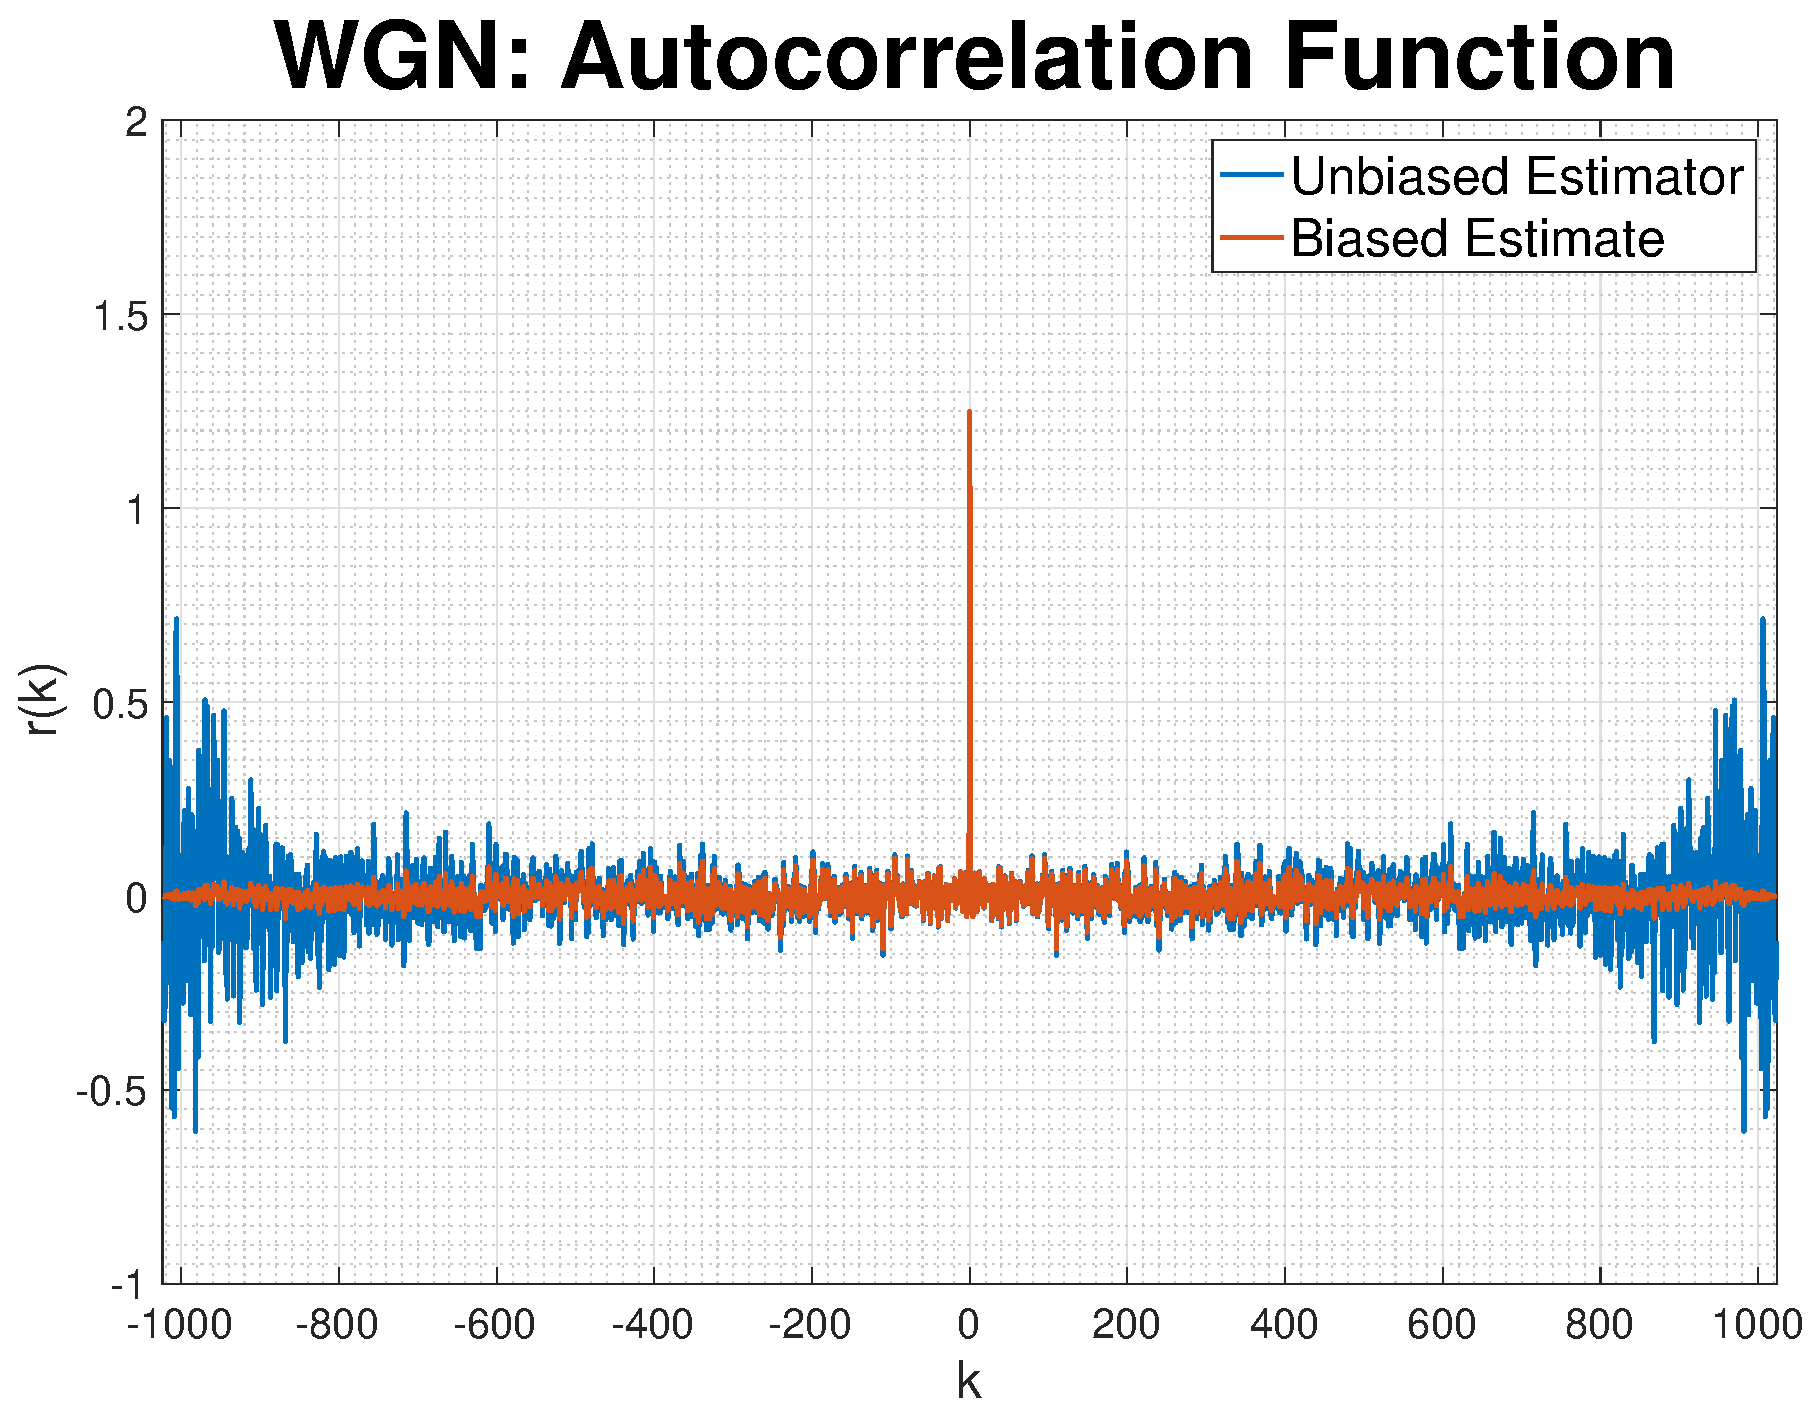
\includegraphics[width=0.32\textwidth]{part2/wgn_biased_and_unbiased_estimates}
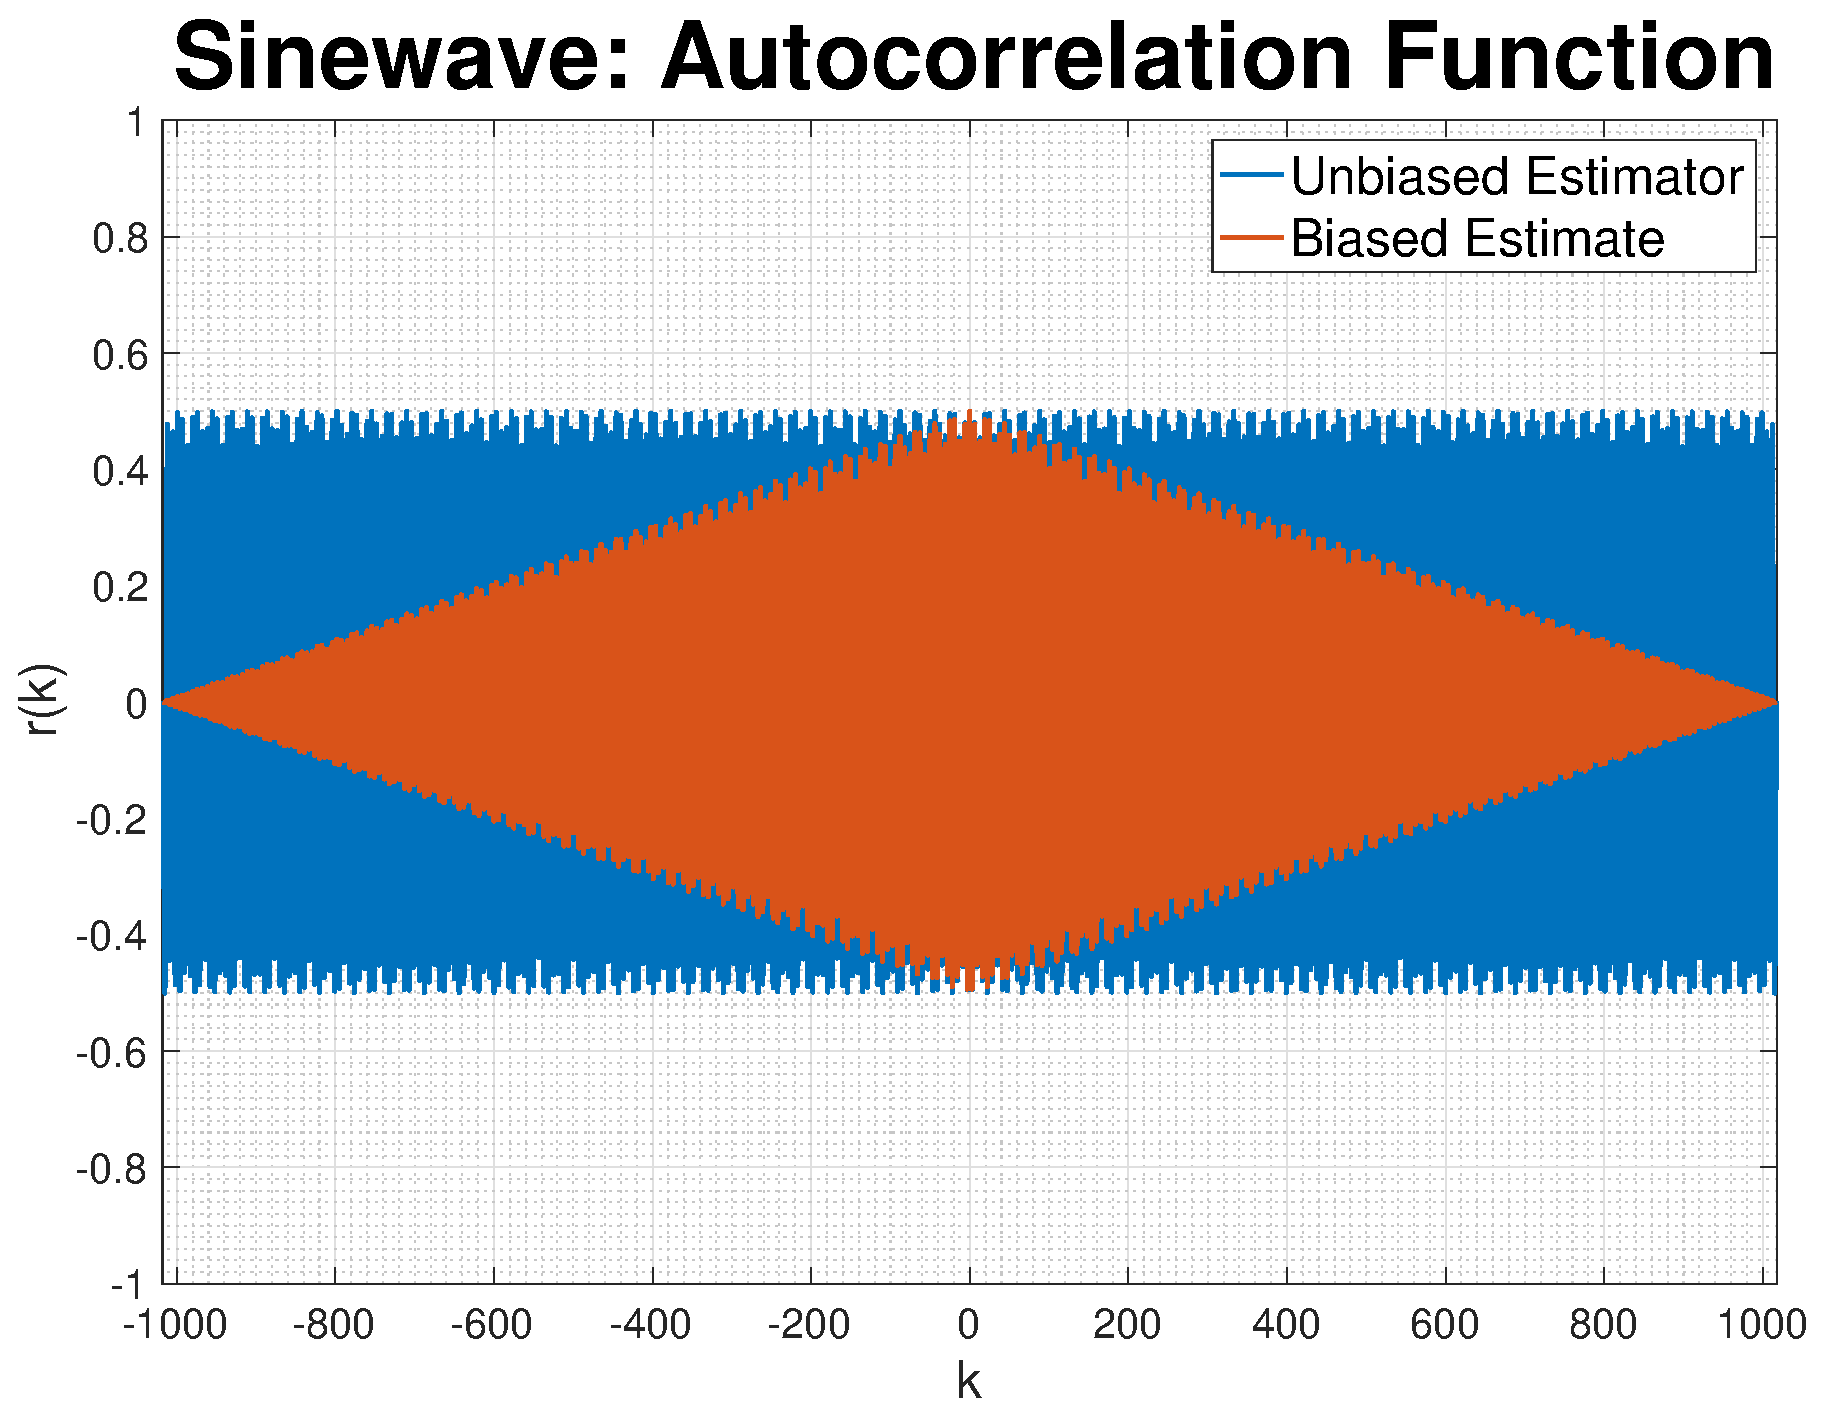
\includegraphics[width=0.32\textwidth]{part2/sinewave_biased_and_unbiased_estimates}
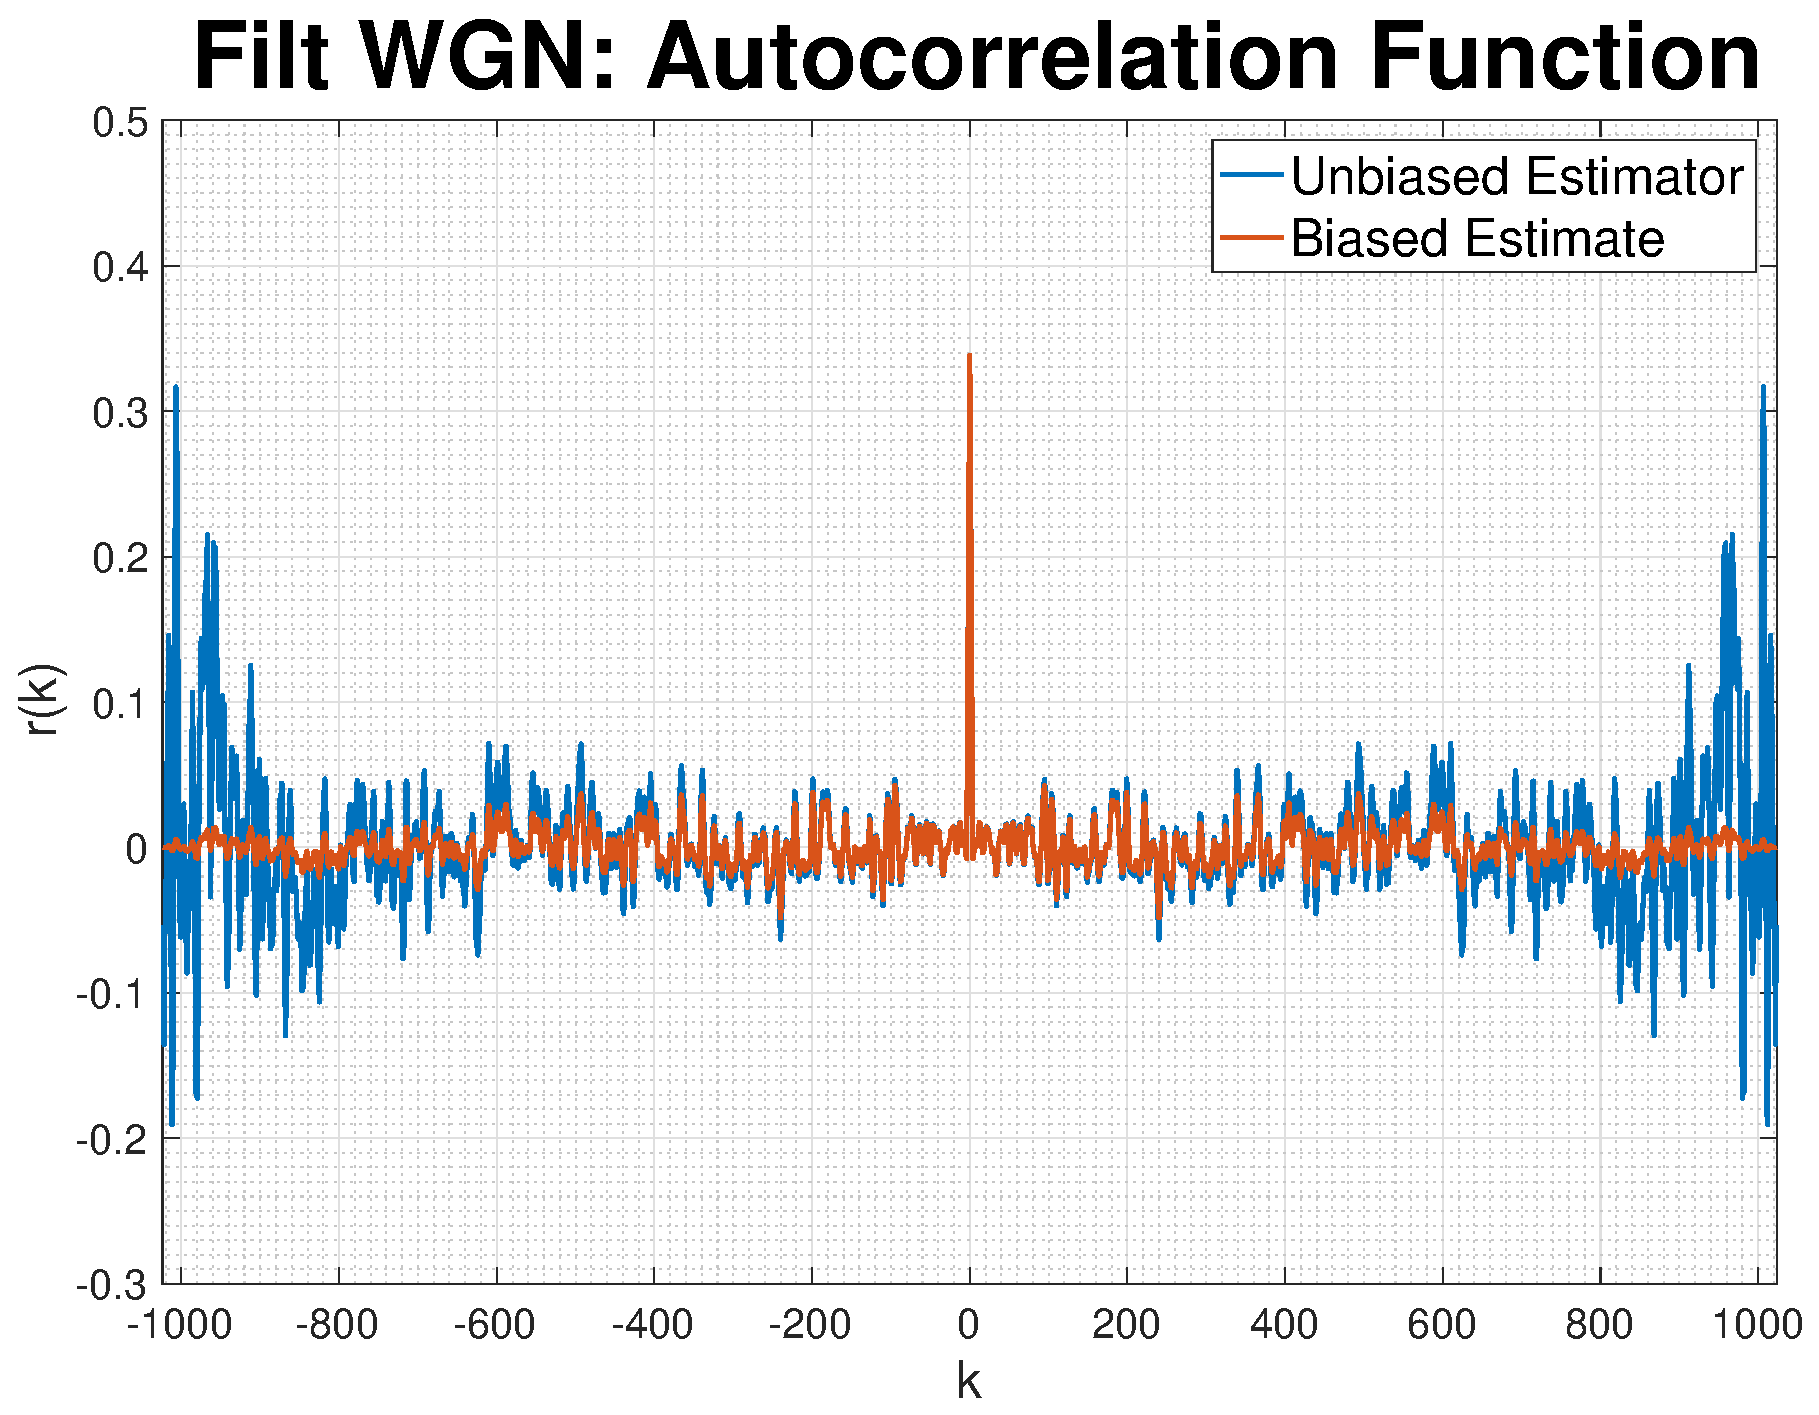
\includegraphics[width=0.32\textwidth]{part2/filt_wgn_biased_and_unbiased_estimates}
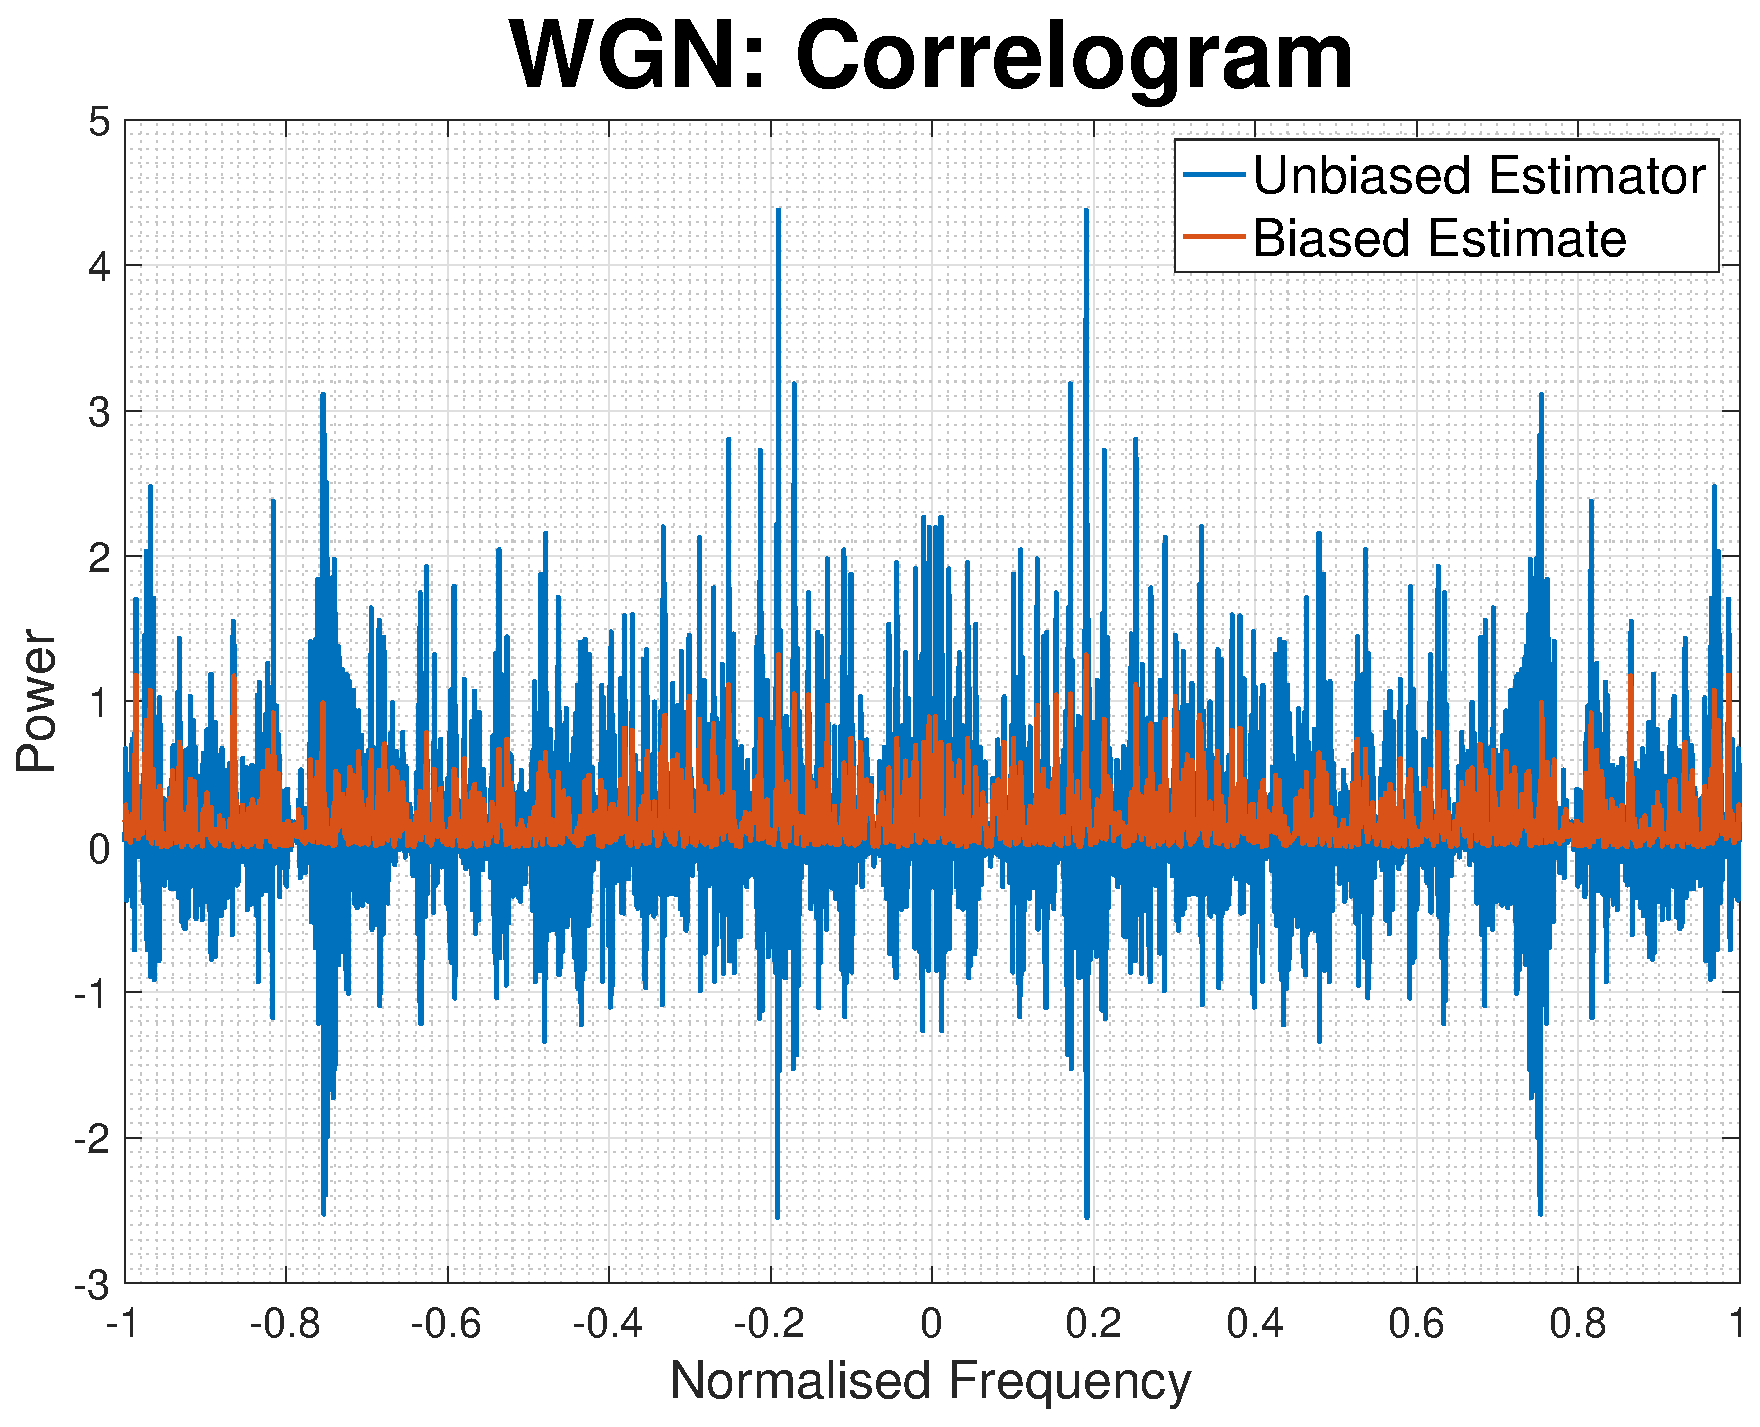
\includegraphics[width=0.32\textwidth]{part2/wgn_correlogram}
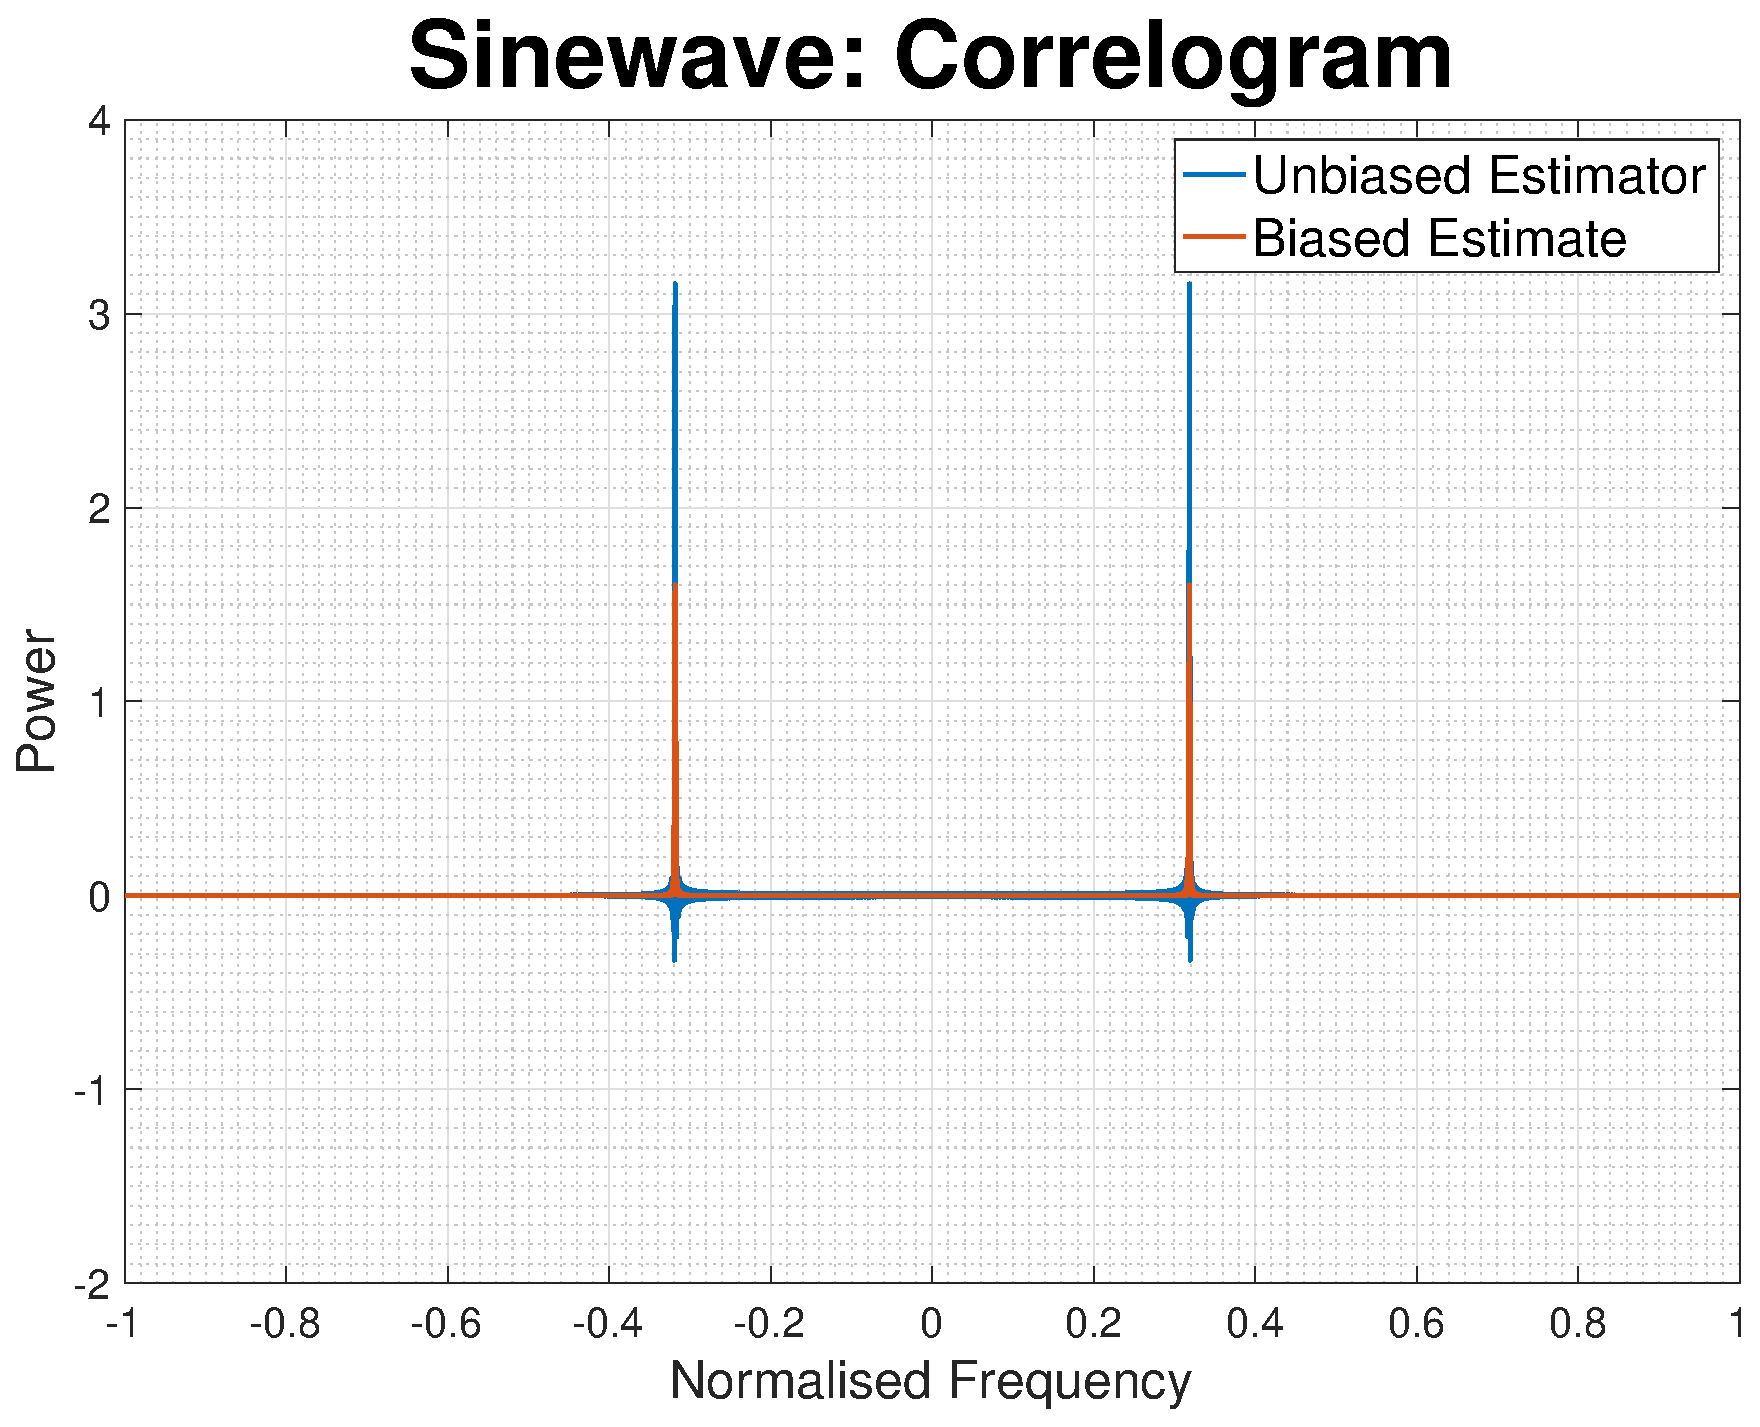
\includegraphics[width=0.32\textwidth]{part2/sinewave_correlogram}
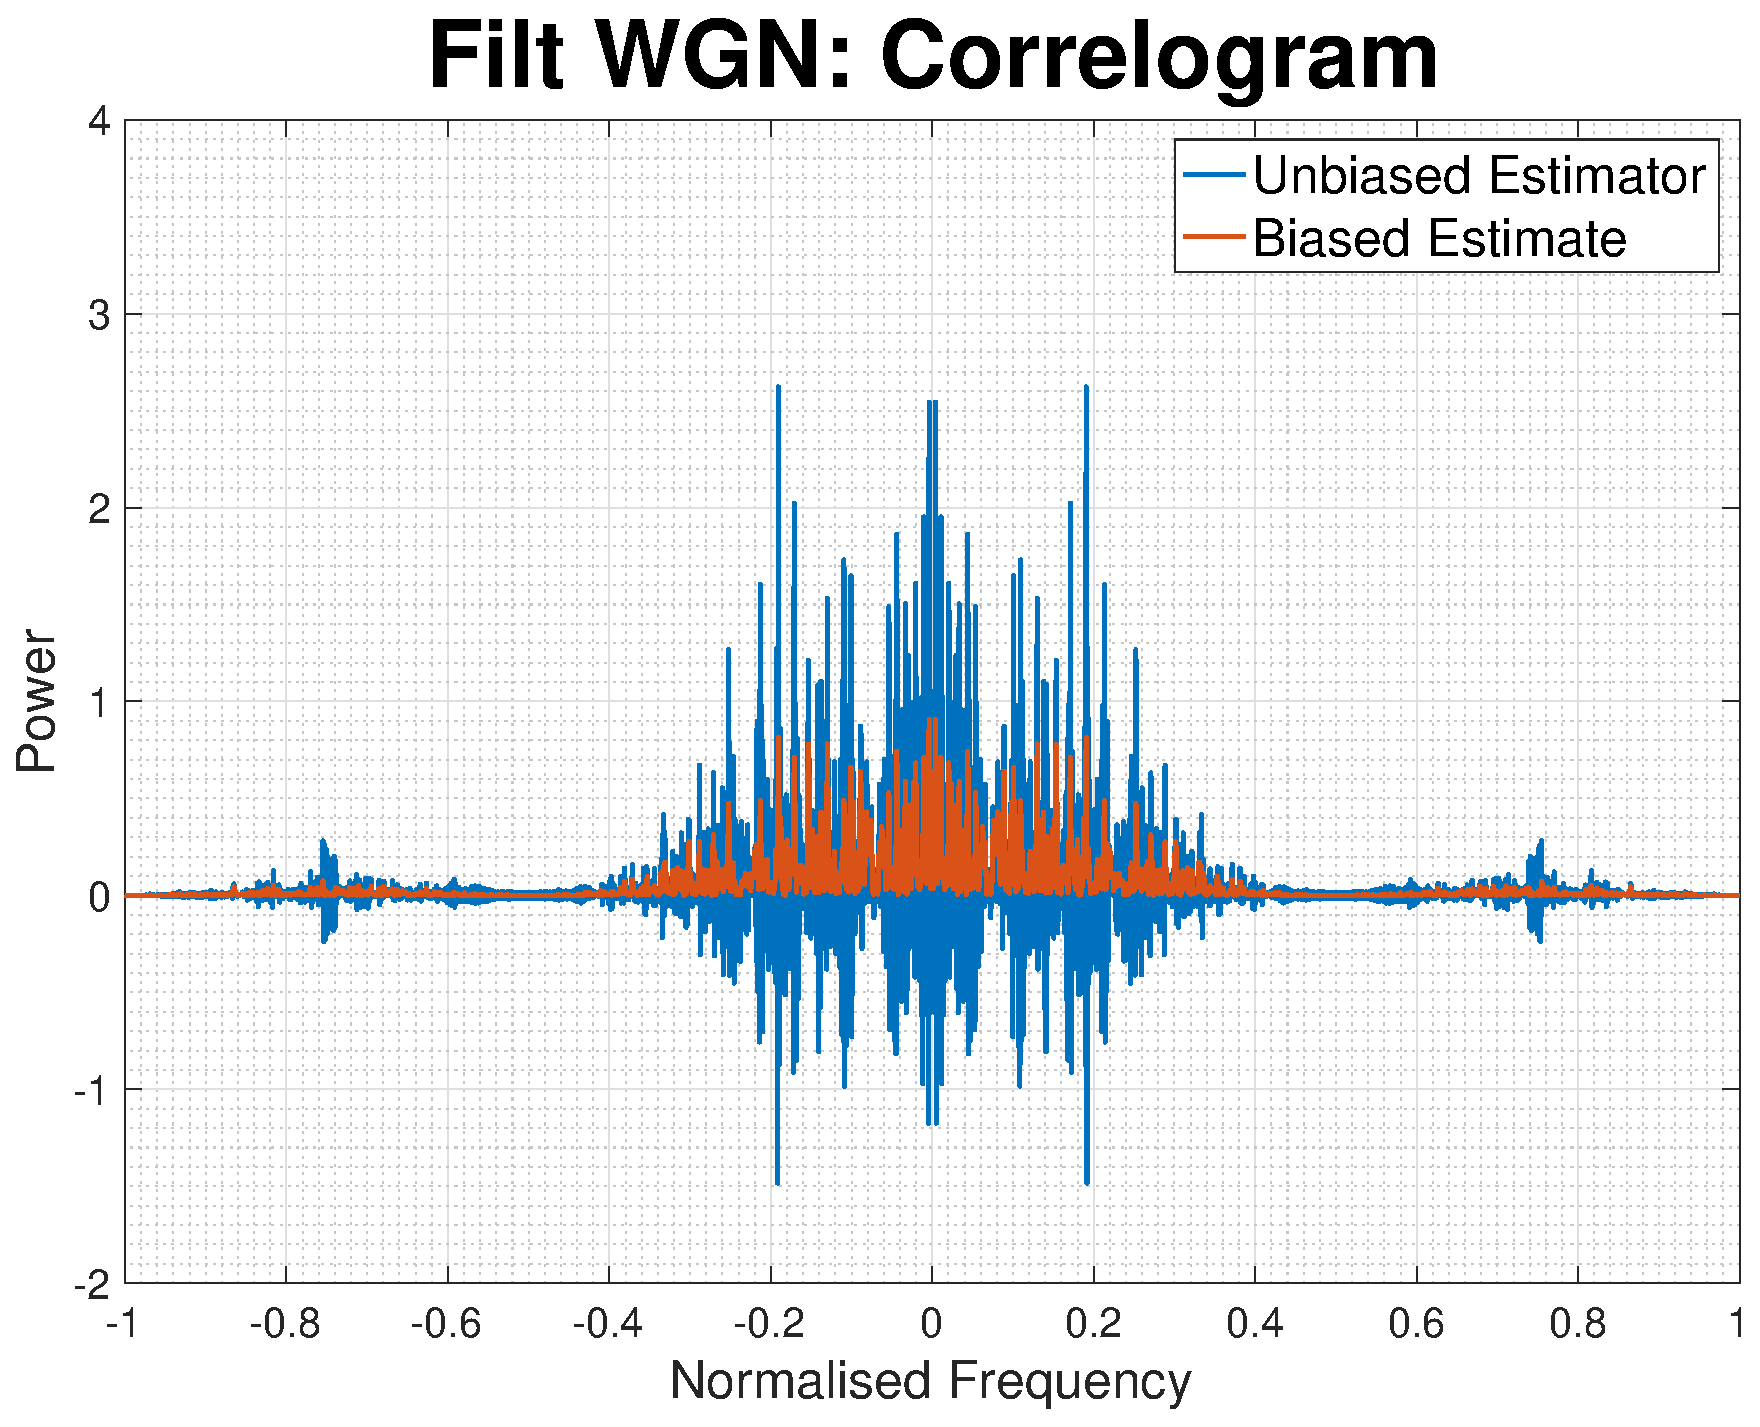
\includegraphics[width=0.32\textwidth]{part2/filt_wgn_correlogram}
\caption{Biased and Unbiased Estimates of ACF and their Effect on the Correlogram}
\end{figure}

\begin{figure}[H]
\centering{}
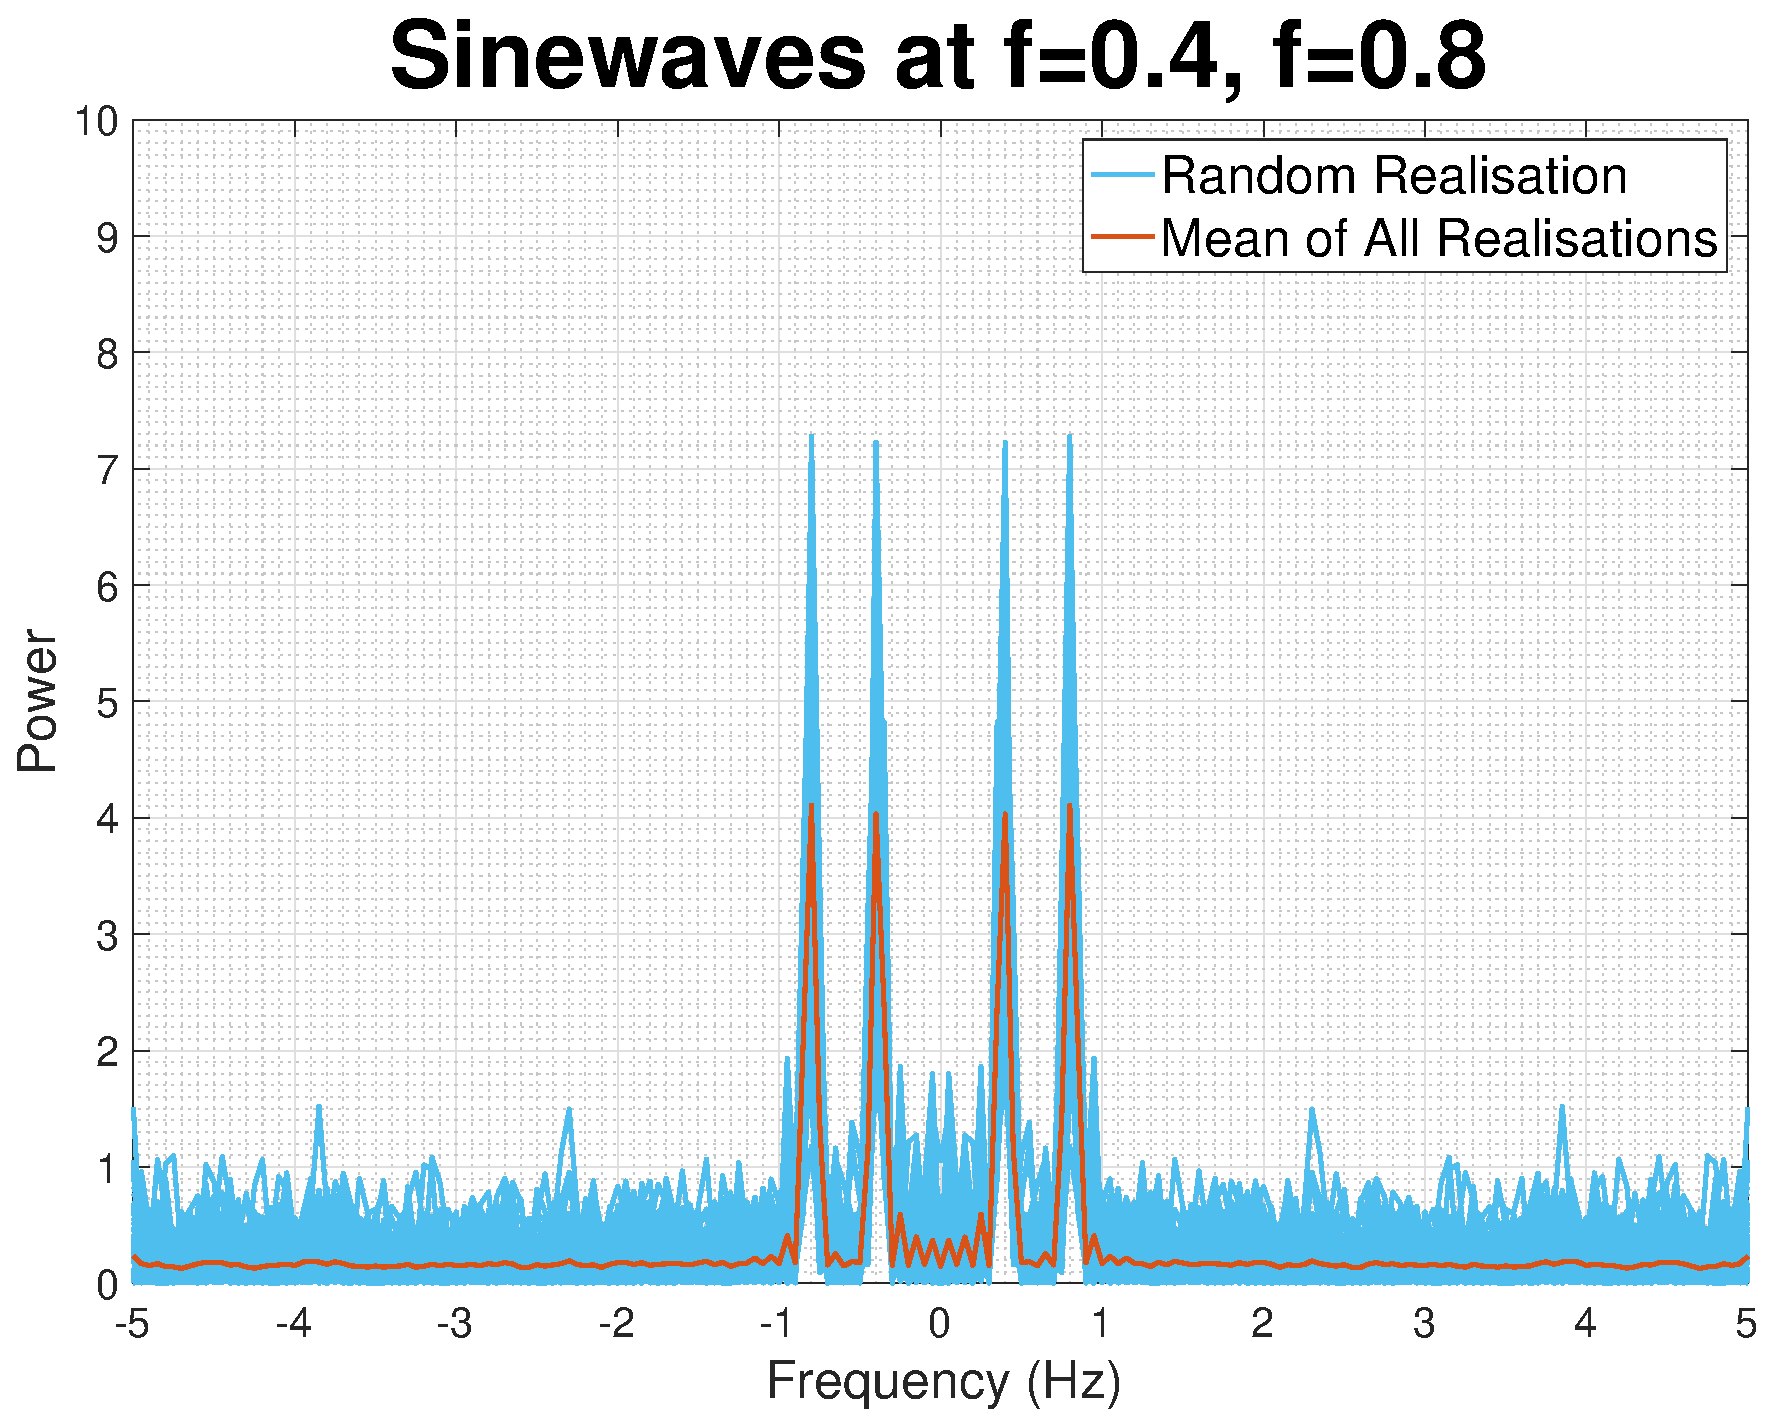
\includegraphics[width=0.32\textwidth]{part2/variance_correlogram_sine_waves_4_8}
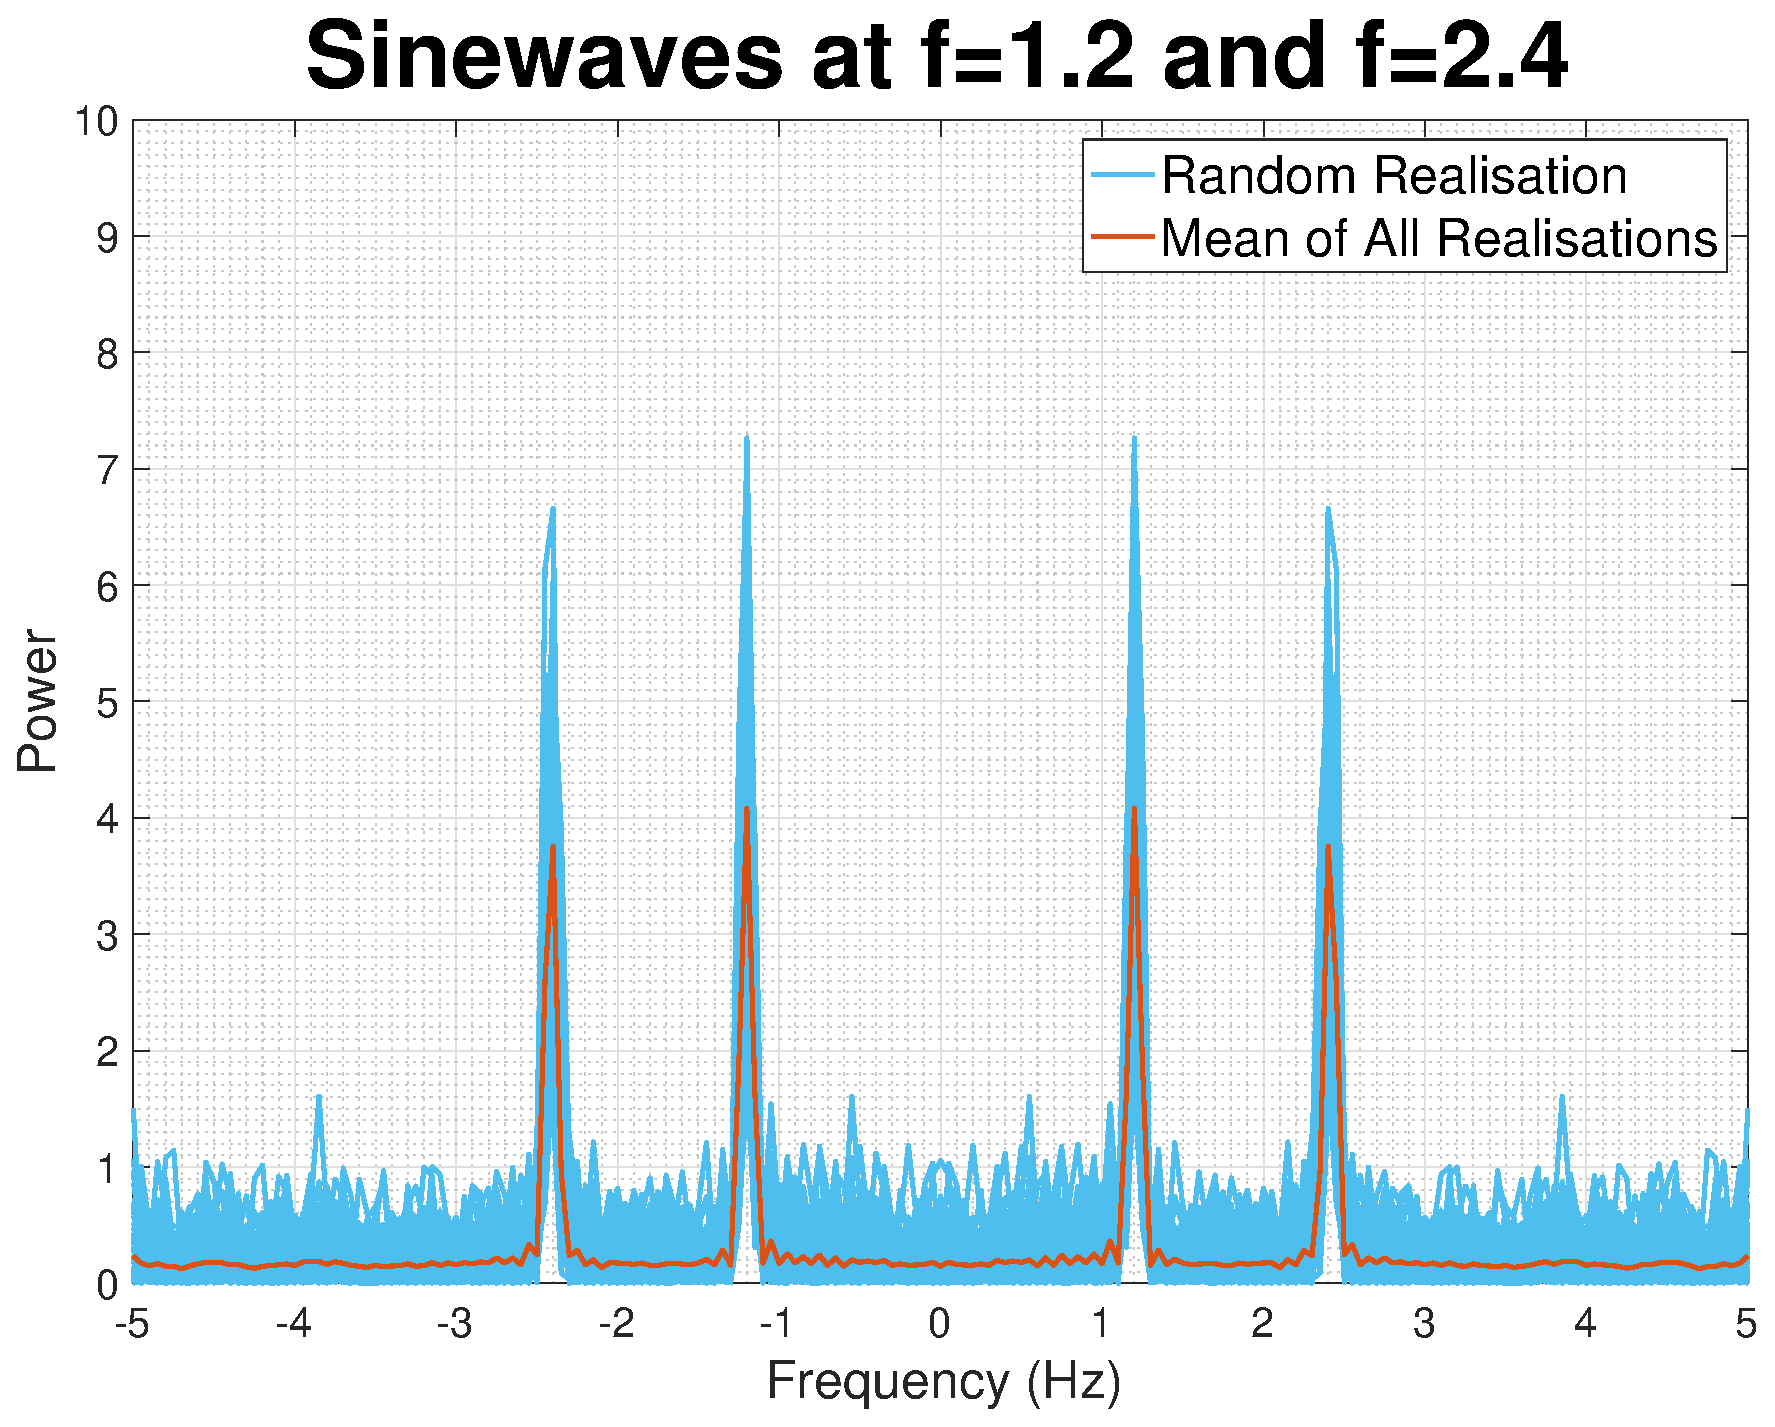
\includegraphics[width=0.32\textwidth]{part2/variance_correlogram_sine_waves_1_2} \\
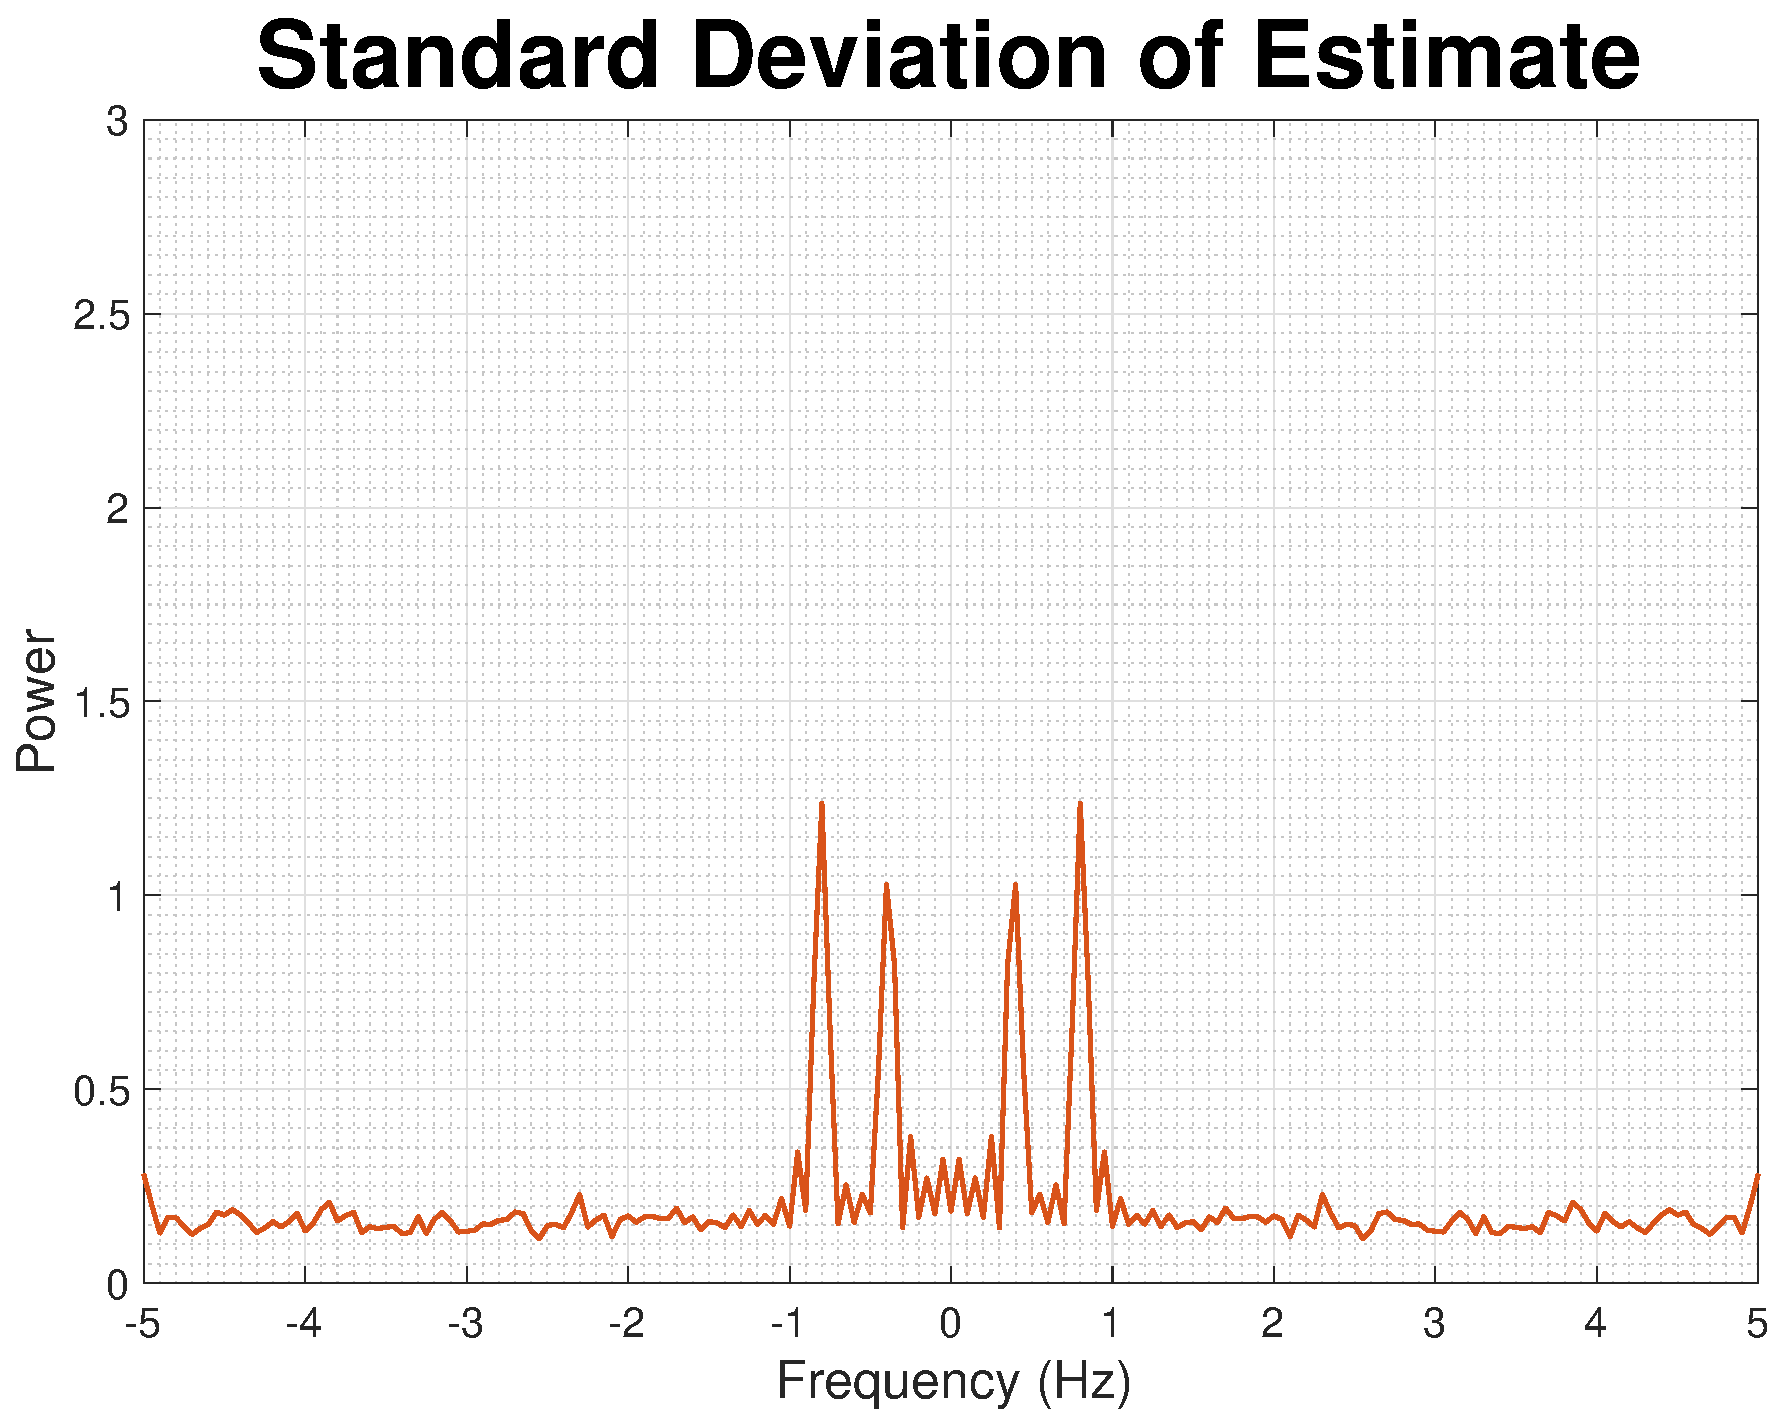
\includegraphics[width=0.32\textwidth]{part2/std_dev_correlogram_sine_waves_4_8}
\includegraphics[width=0.32\textwidth]{part2/std_dev_correlogram_sine_waves_1_2}
\caption{Variance and Standard Deviation of Correlogram Spectral Estimates}
\end{figure}

\begin{figure}[H]
\centering{}
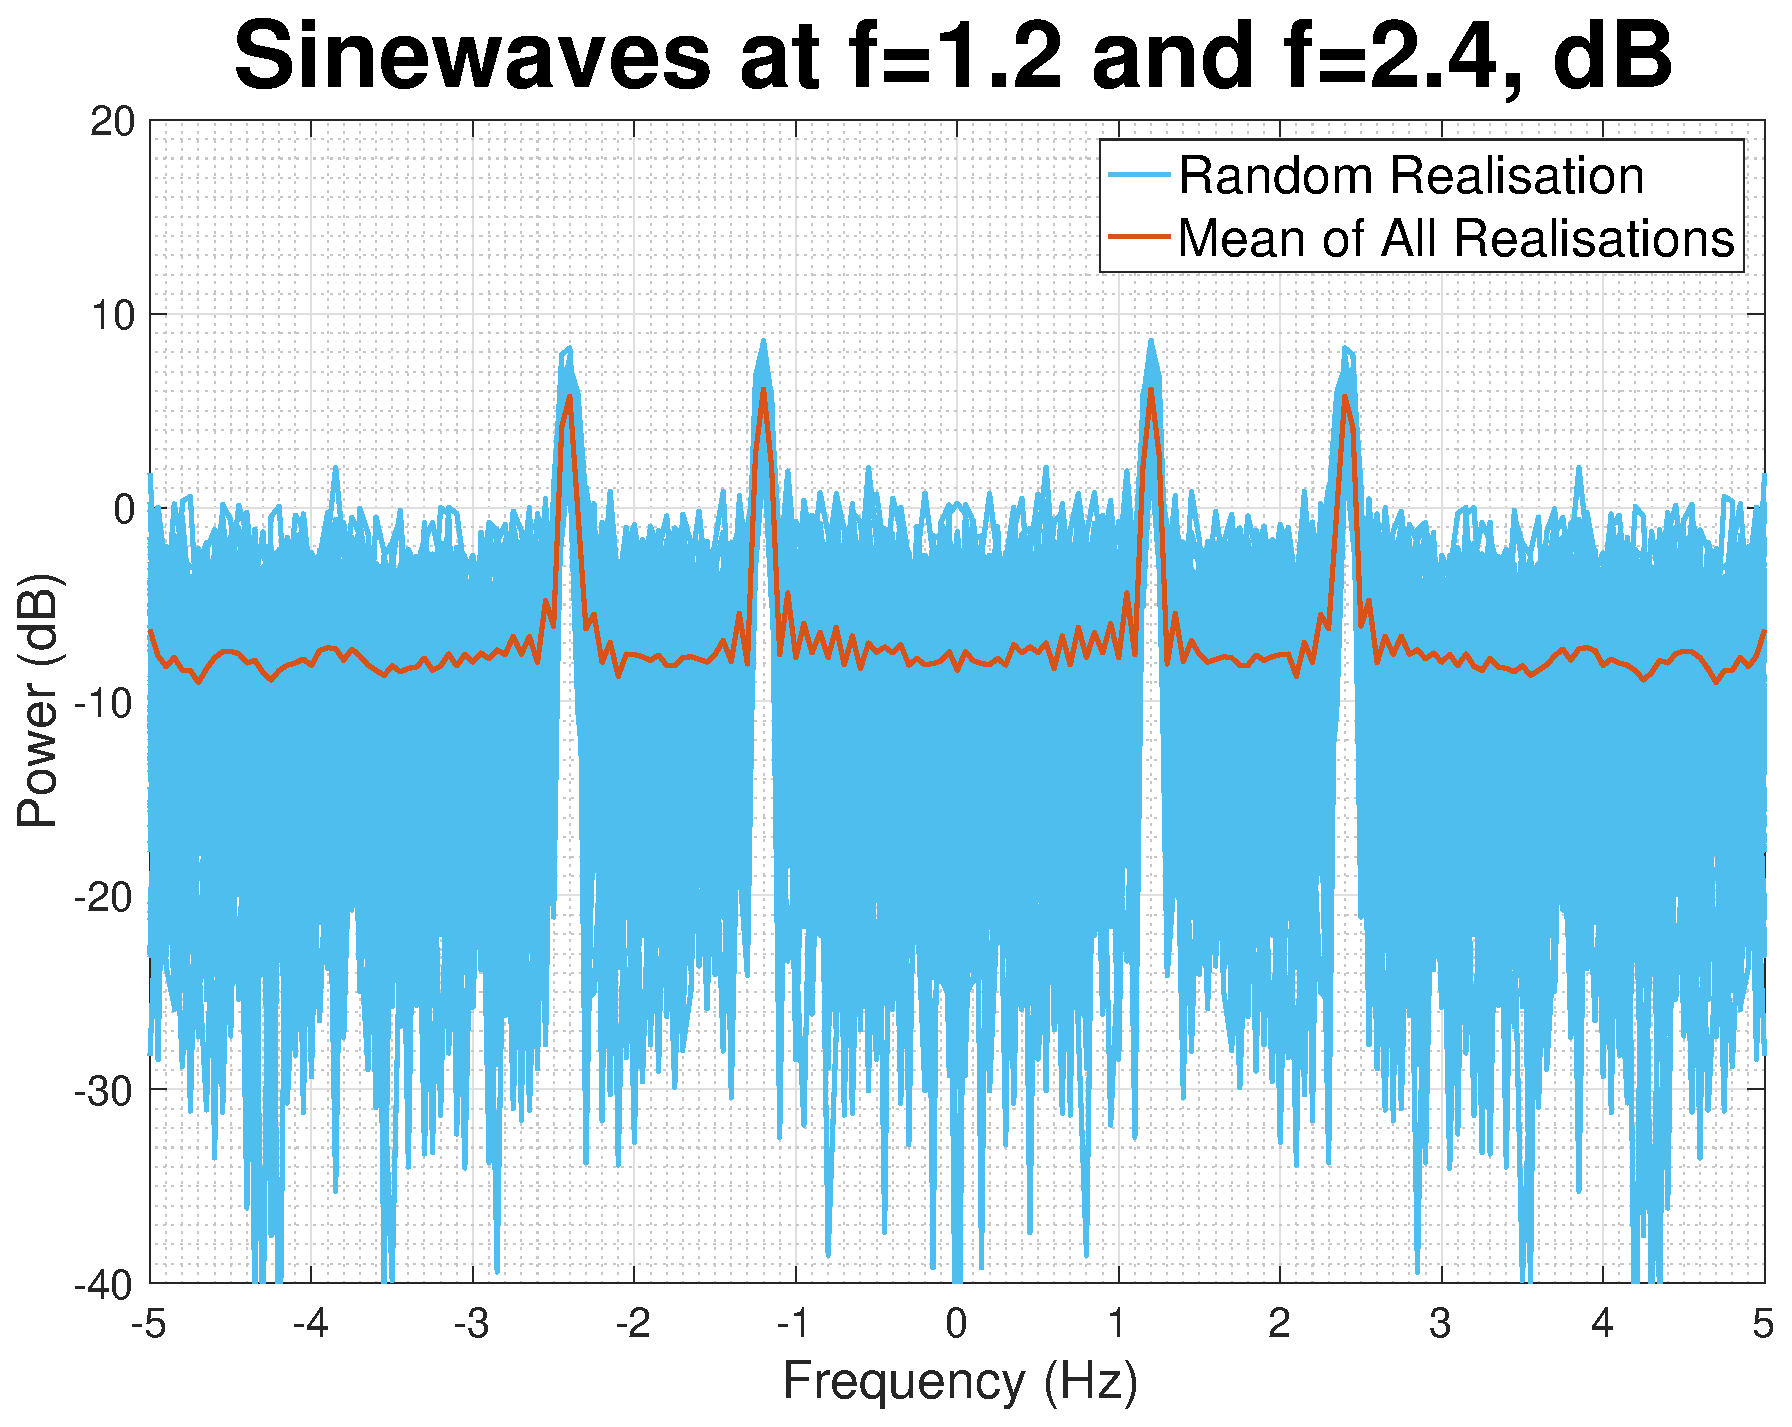
\includegraphics[width=0.32\textwidth]{part2/variance_correlogram_sine_waves_1_2_dB}
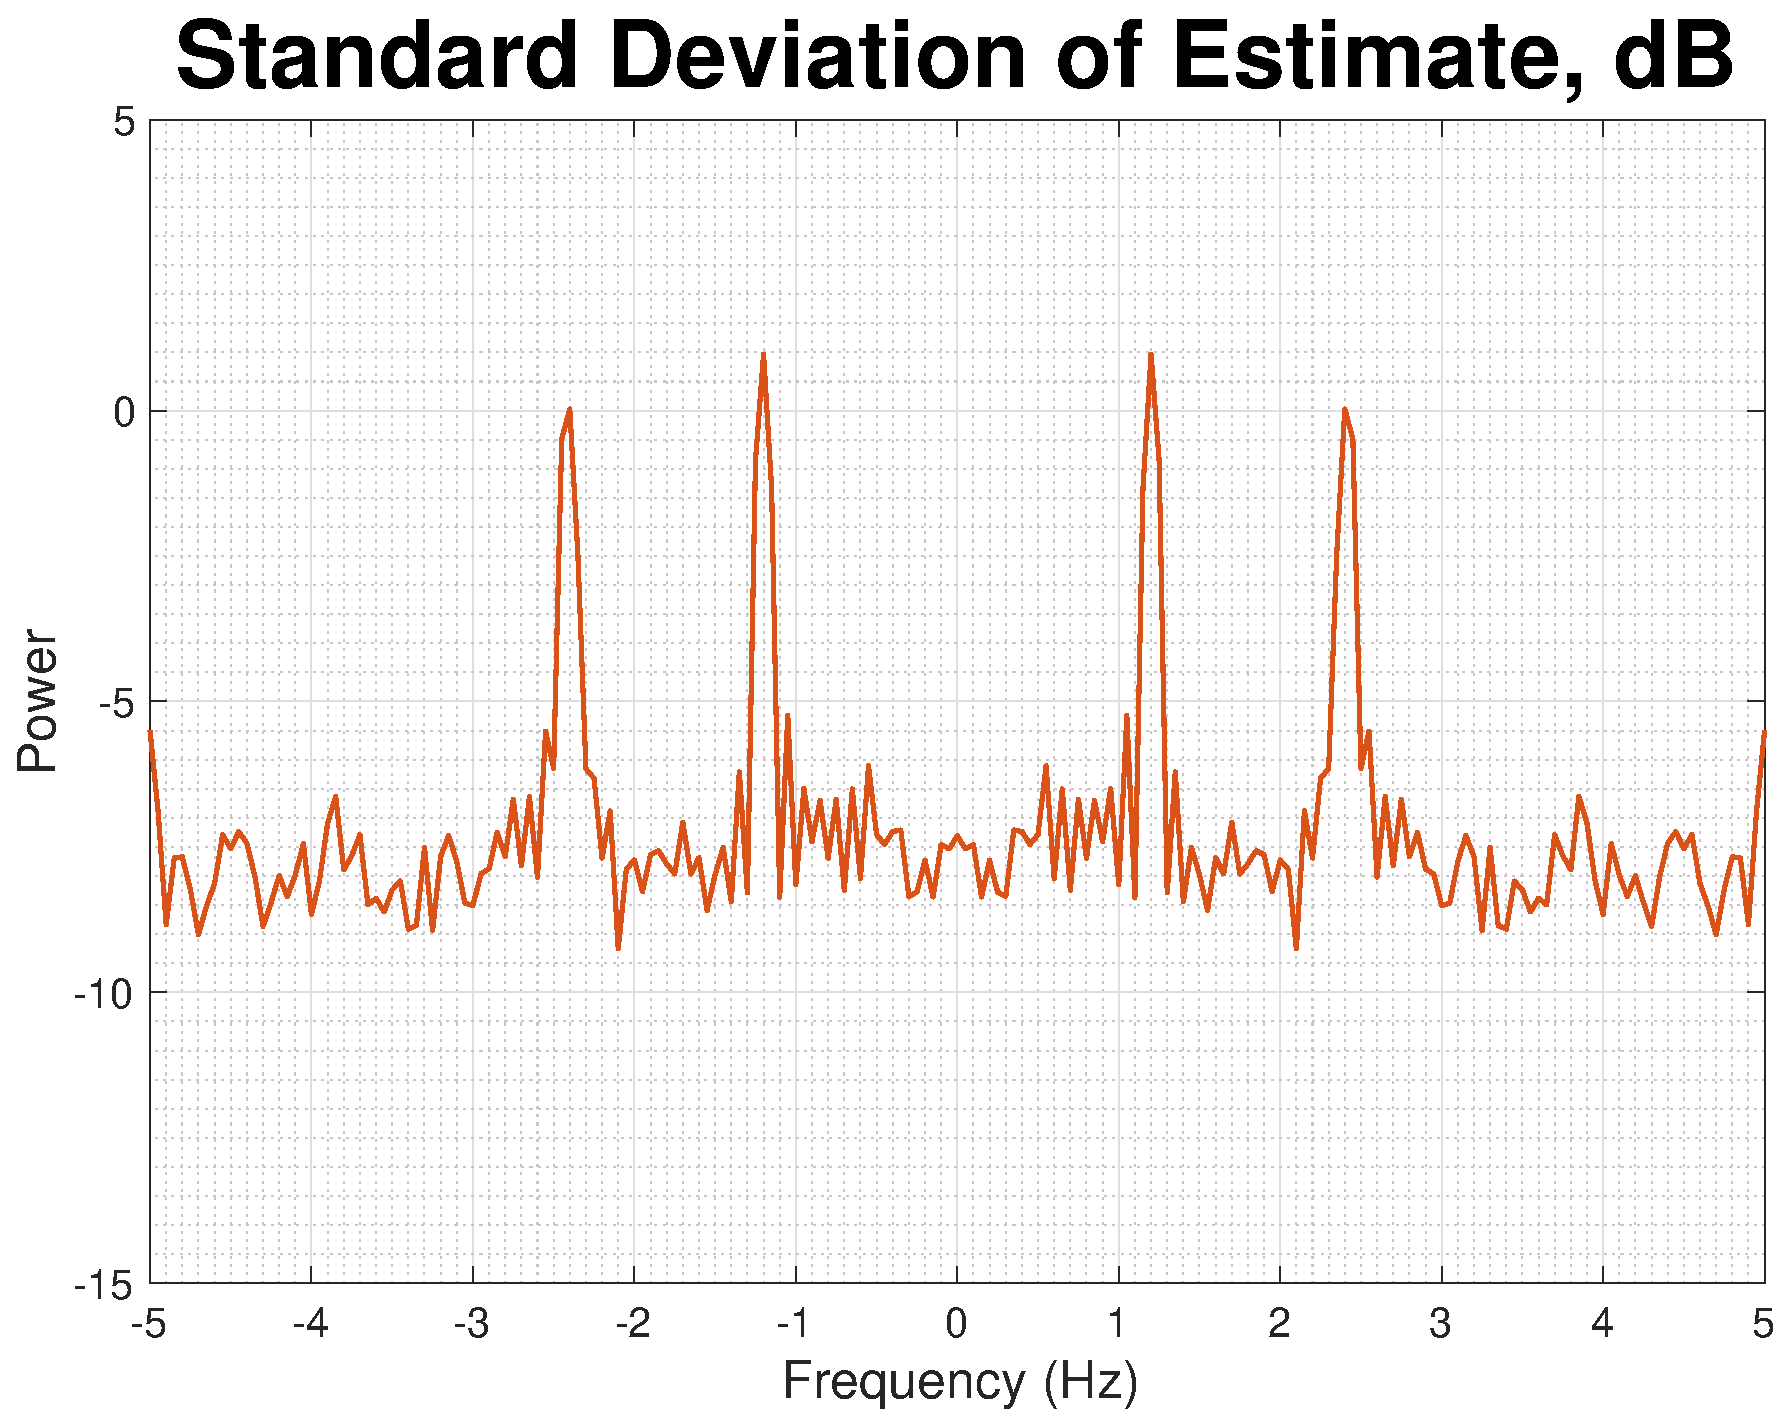
\includegraphics[width=0.32\textwidth]{part2/std_dev_correlogram_sine_waves_1_2_dB}
\caption{Effect of dB Scale on Spread of Variance and Standard Deviation of Correlogram Spectral Estimates}
\end{figure}


\begin{figure}[H]
\centering{}
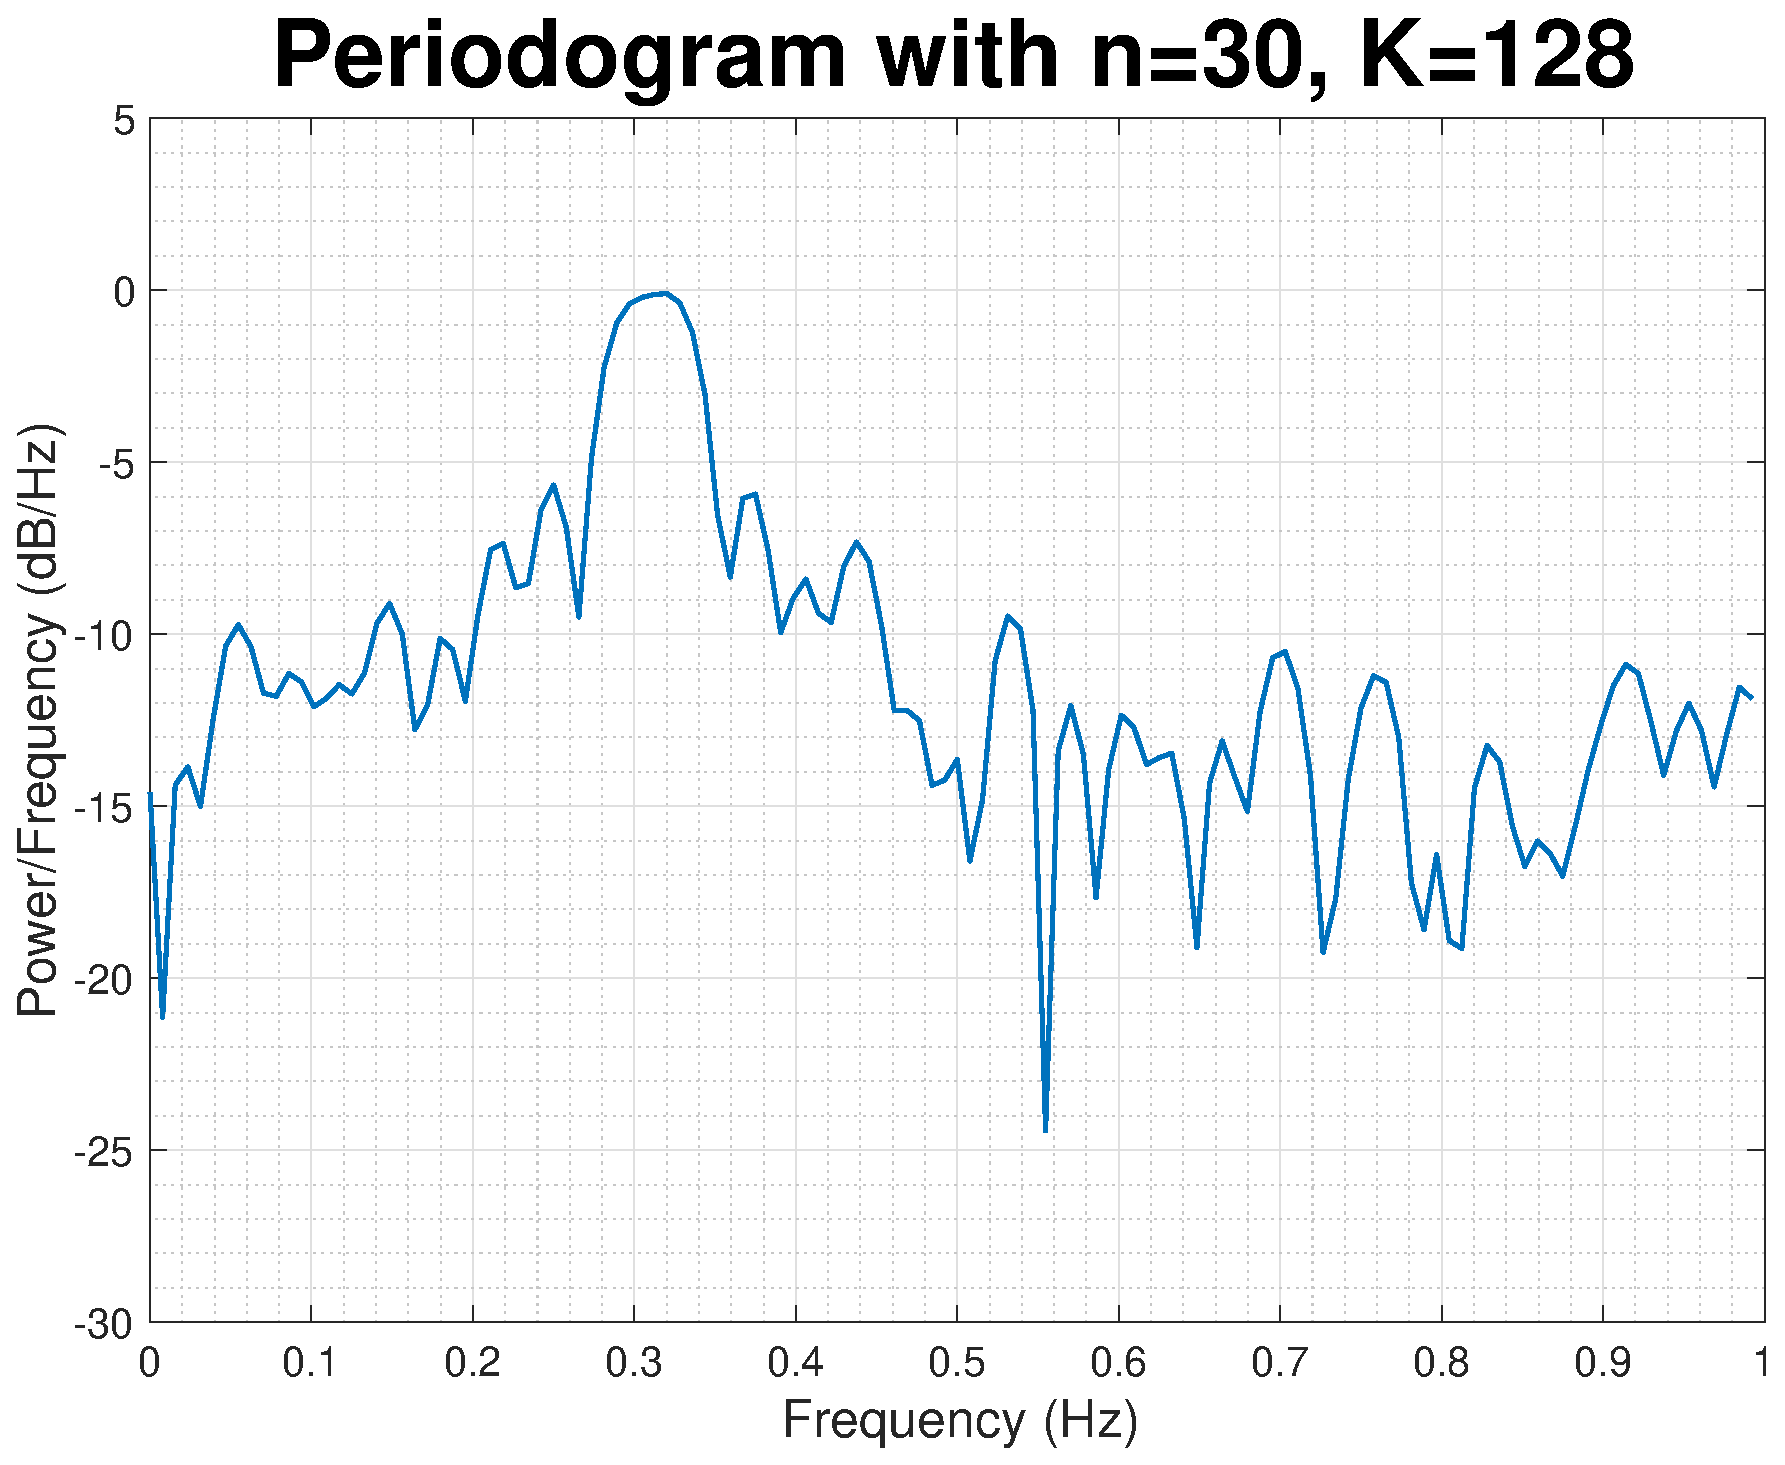
\includegraphics[width=0.32\textwidth]{part2/complex_psd_n_30}
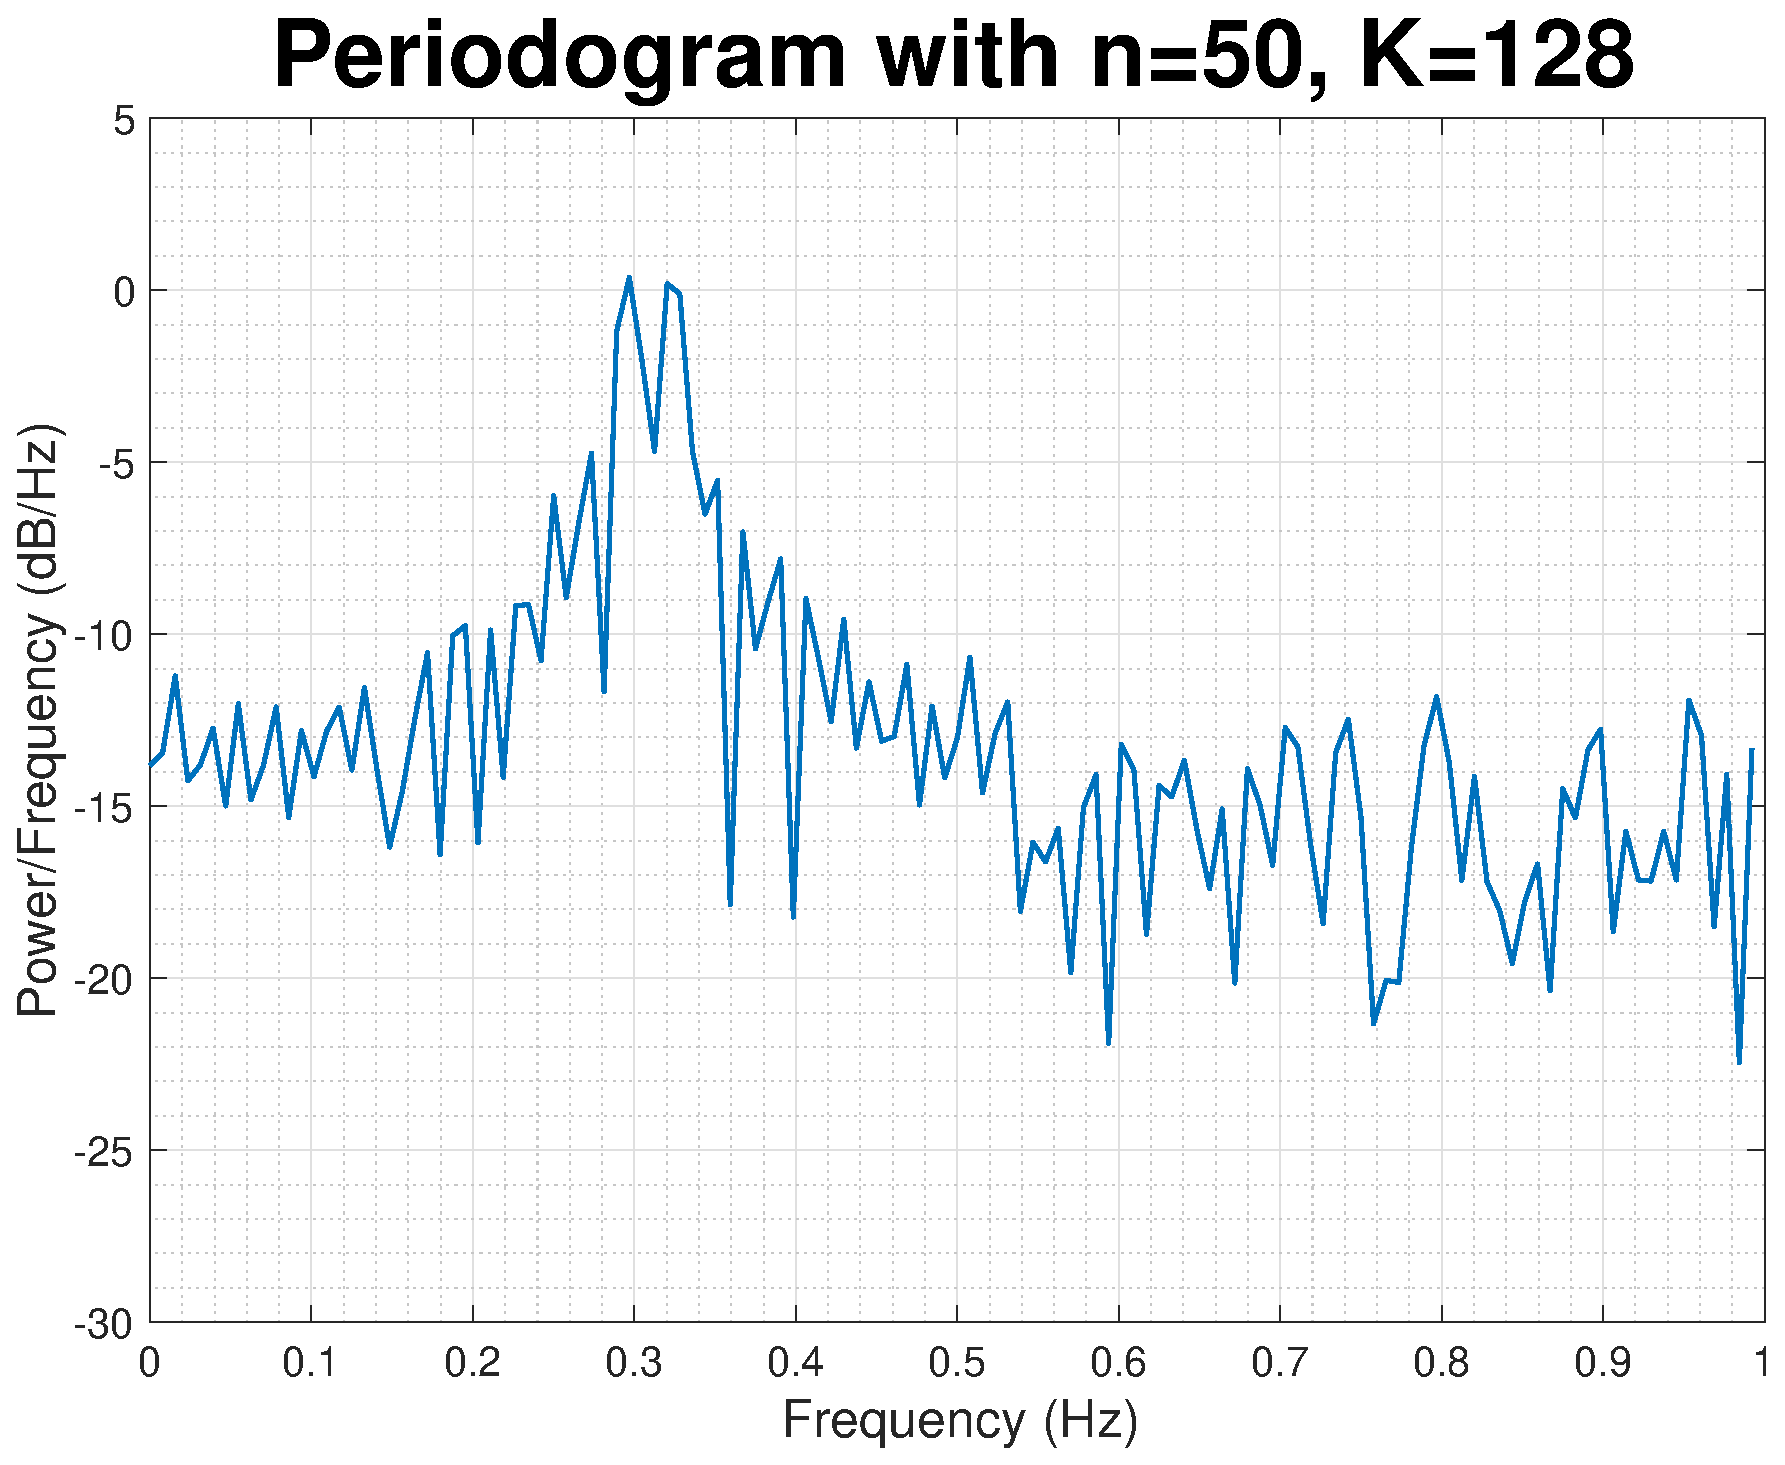
\includegraphics[width=0.32\textwidth]{part2/complex_psd_n_50}
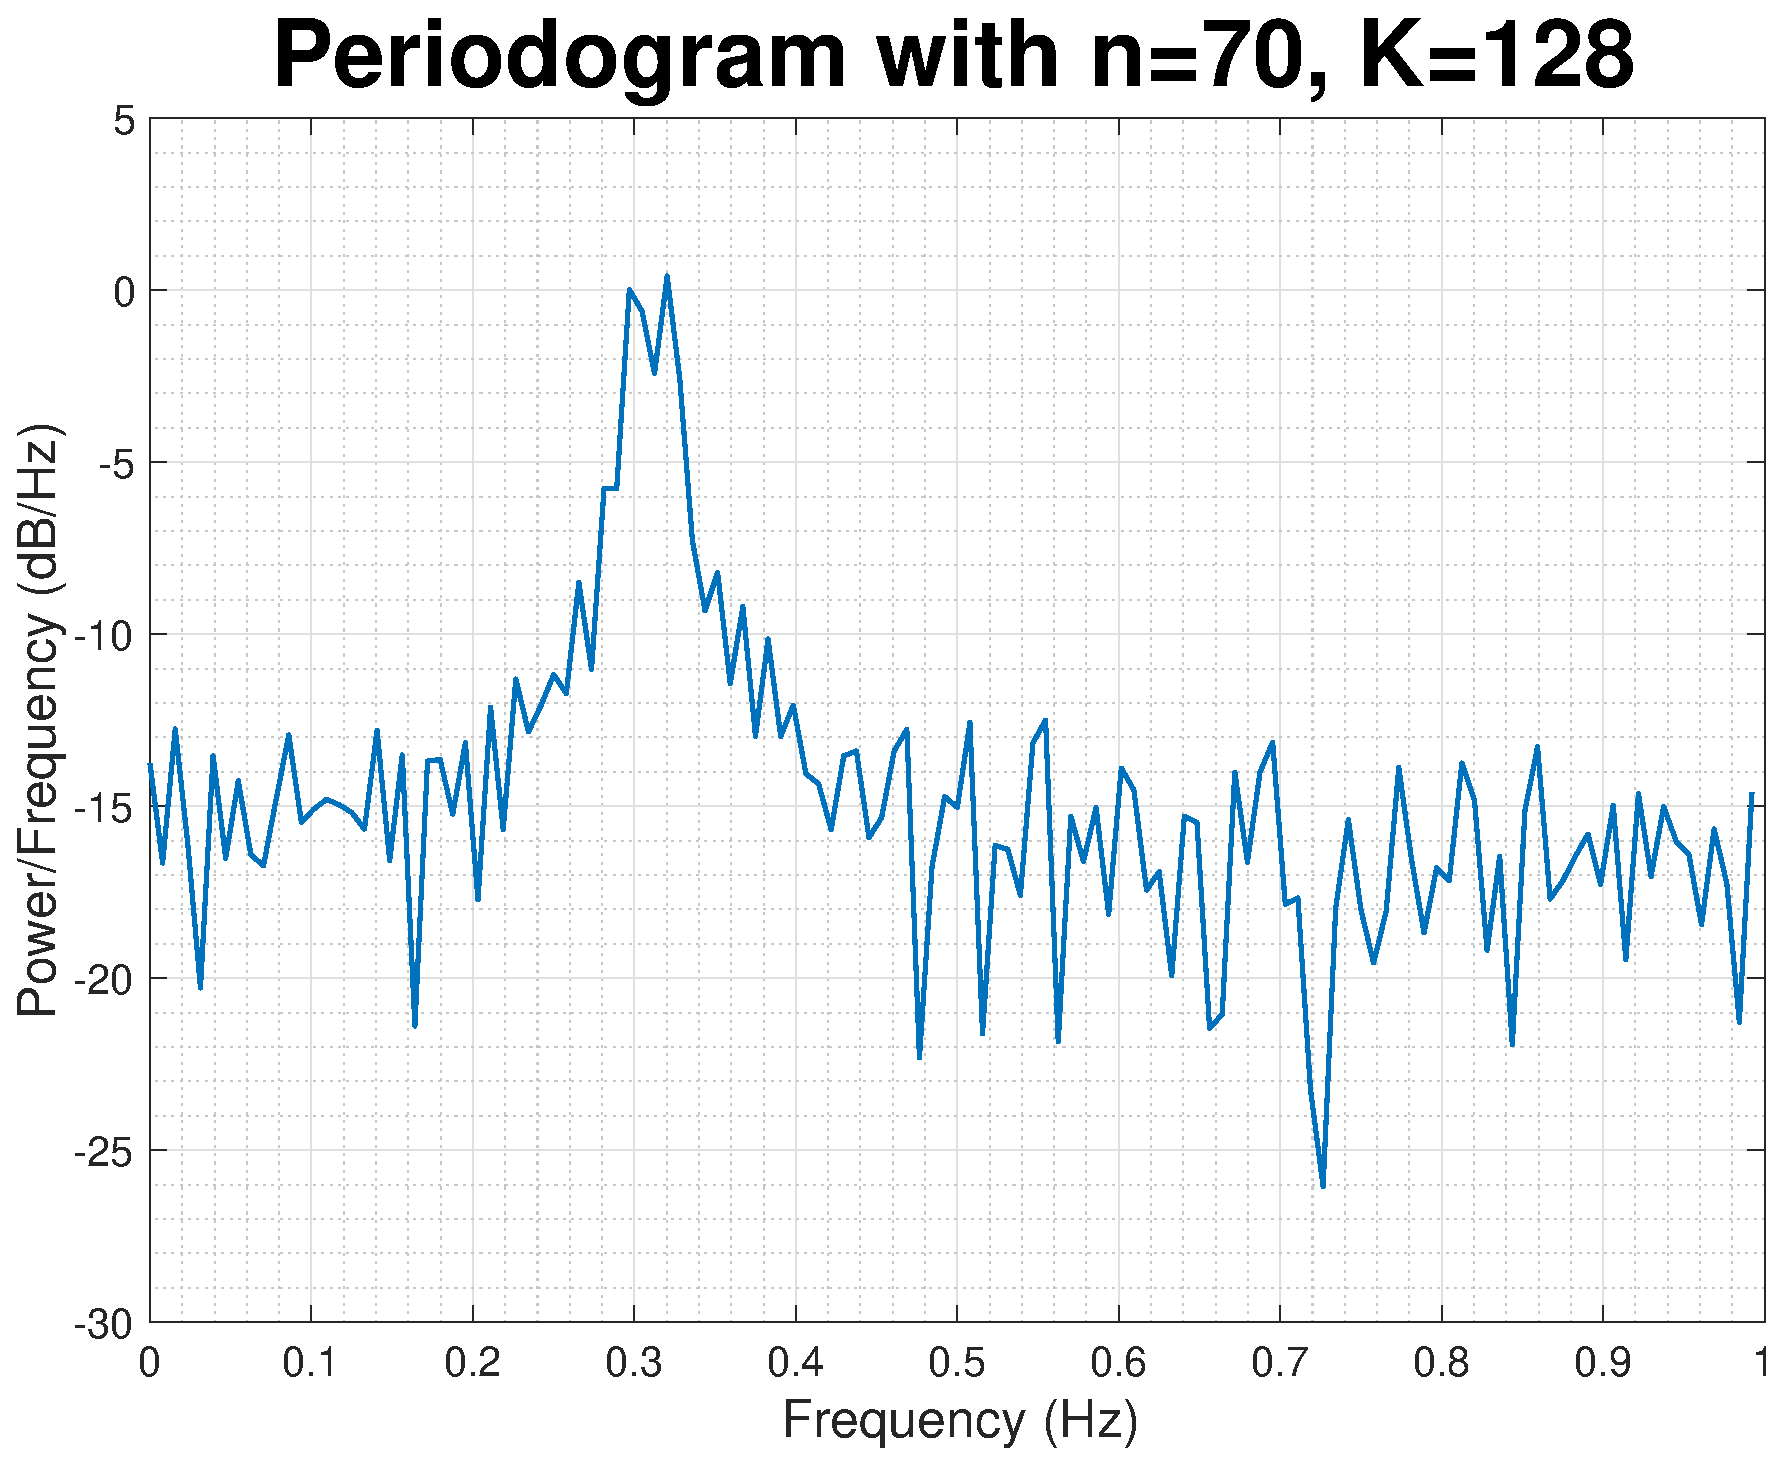
\includegraphics[width=0.32\textwidth]{part2/complex_psd_n_70}
\caption{Effect of Increasing Number of Samples on the Resolution of Periodogram Spectral Estimate}
\end{figure}


\begin{figure}[H]
\centering{}
\includegraphics[width=0.32\textwidth]{part2/music_2_sinewaves_n_30}
\includegraphics[width=0.32\textwidth]{part2/music_3_sine_waves_n_30}
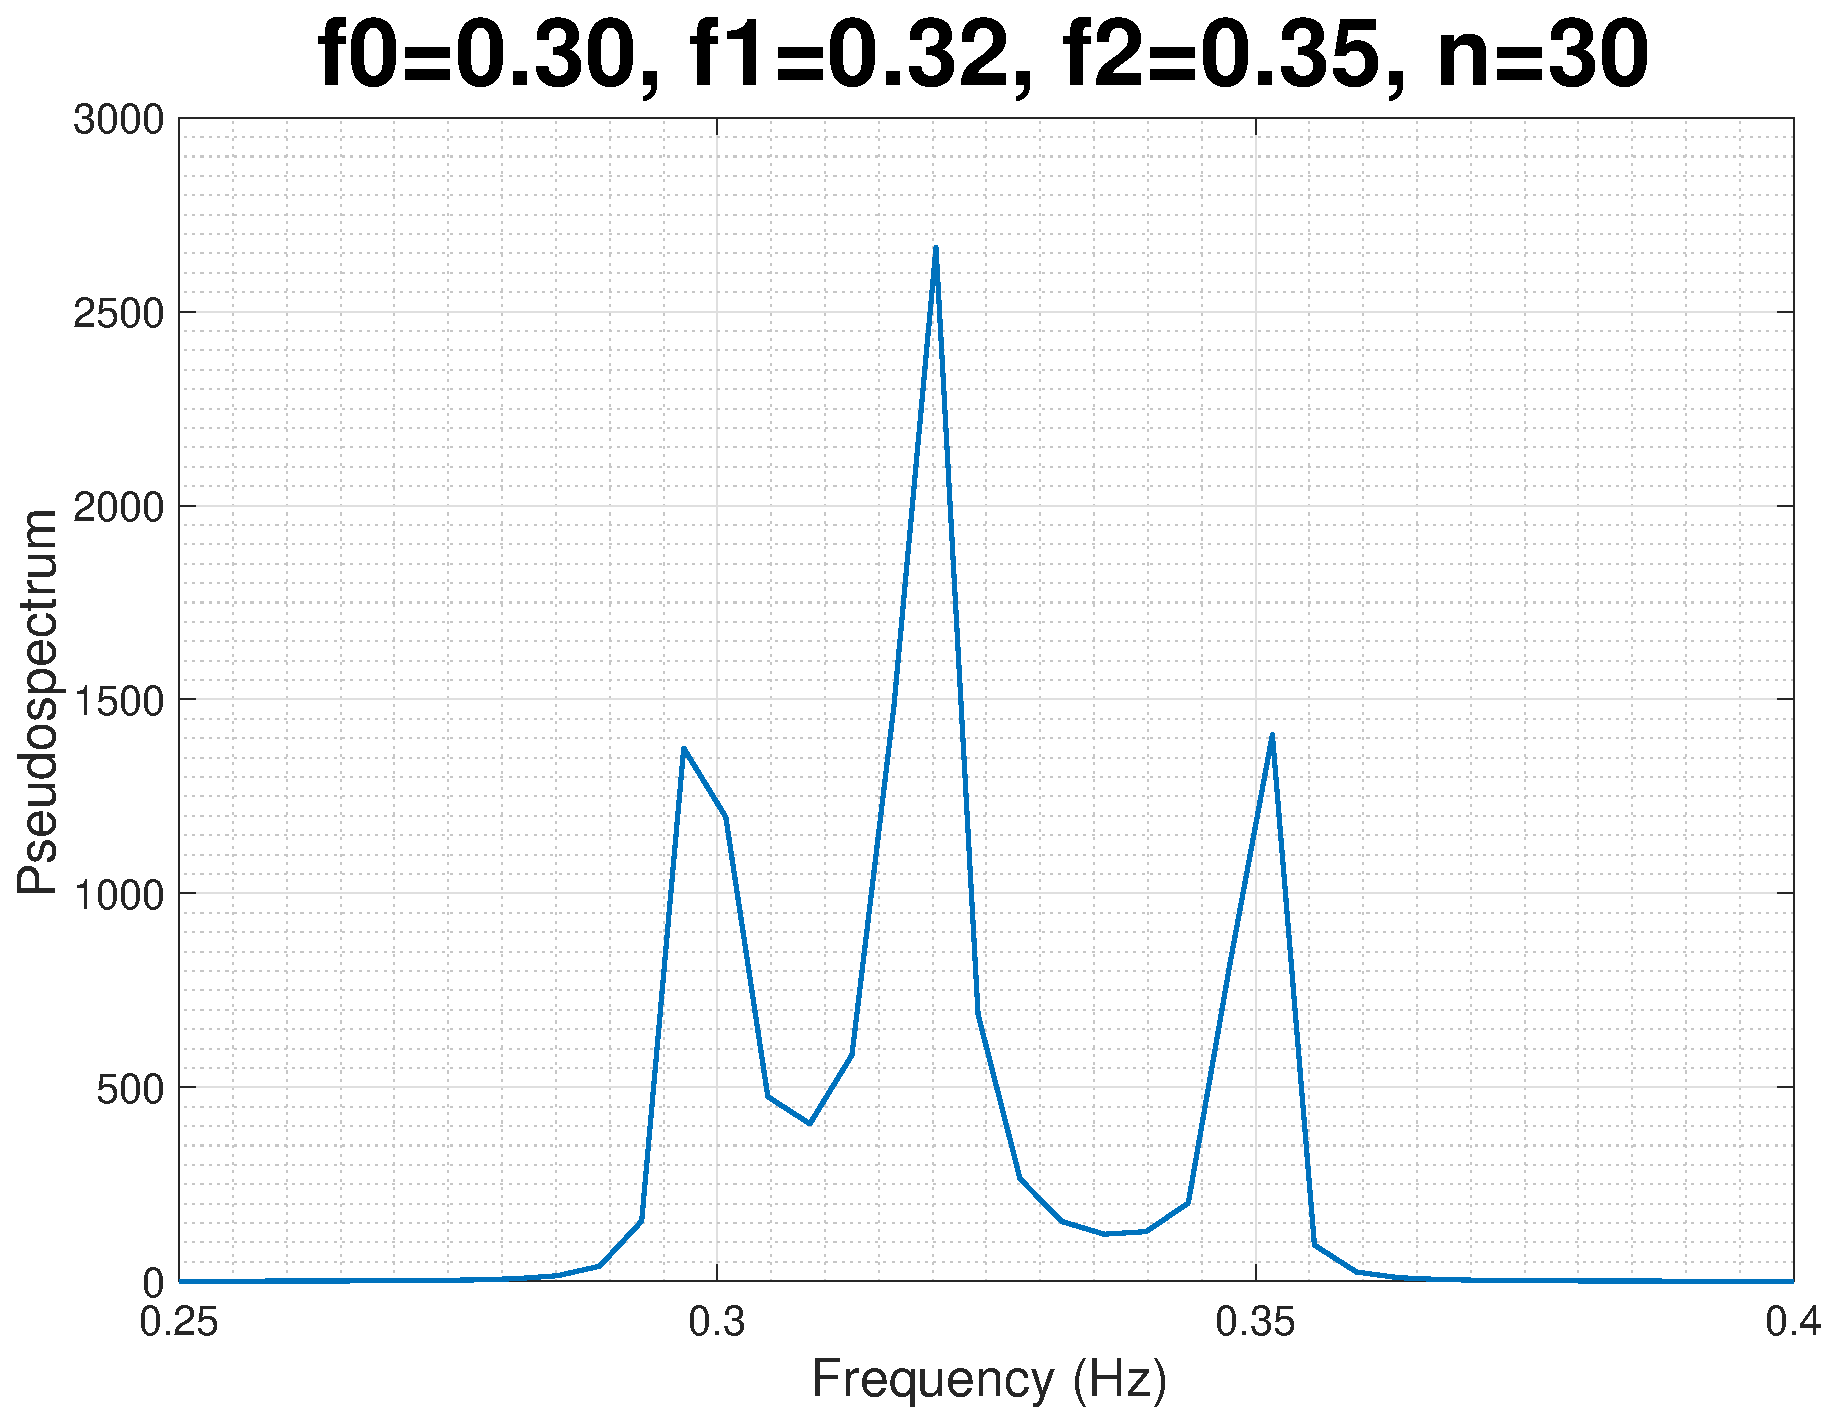
\includegraphics[width=0.32\textwidth]{part2/music_3_sine_waves_n_70}

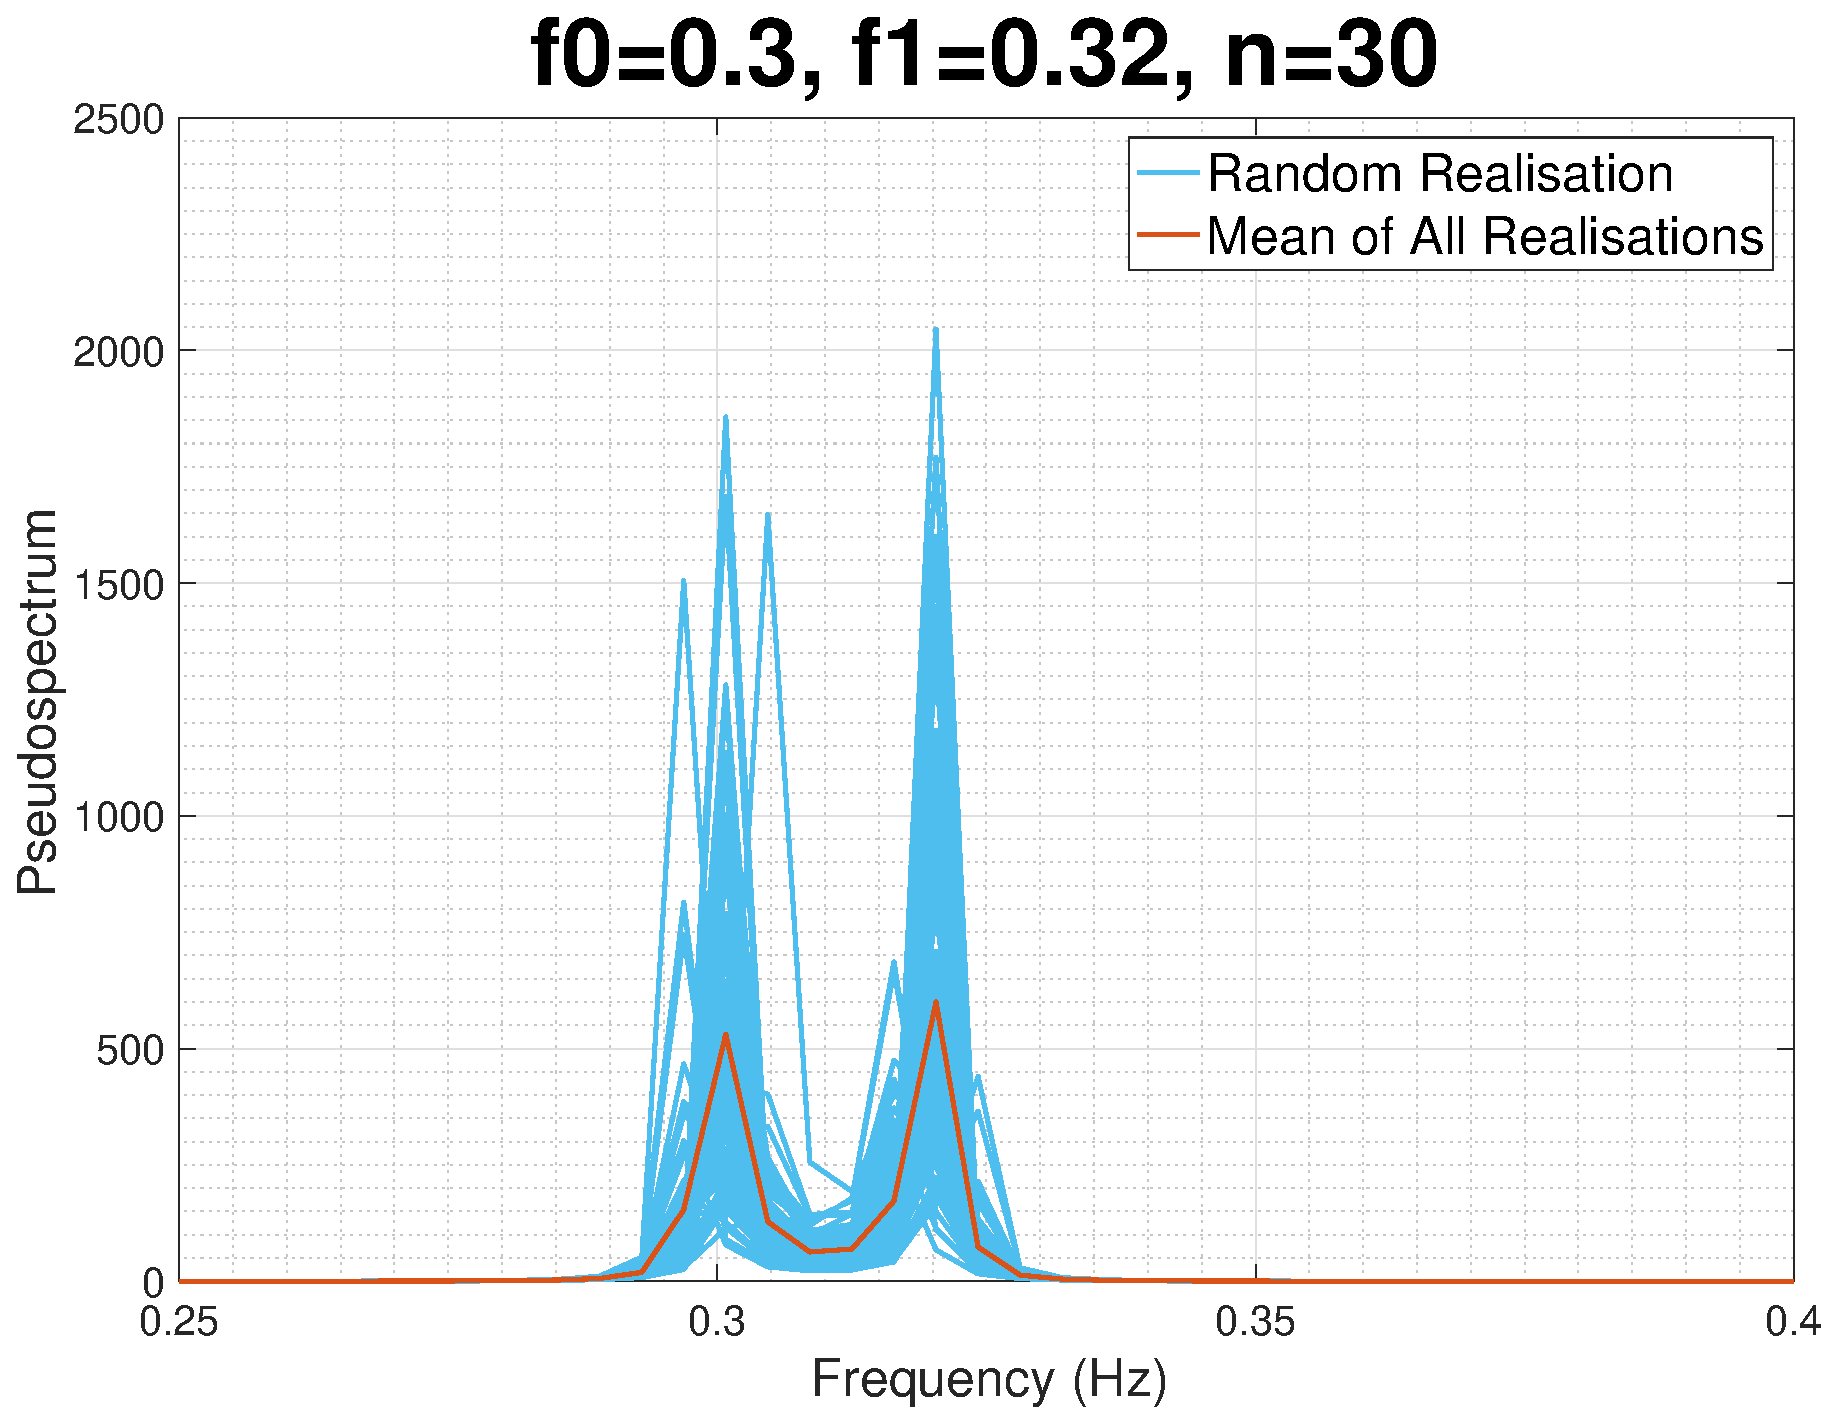
\includegraphics[width=0.32\textwidth]{part2/music_2_sinewaves_n_30_overlay}
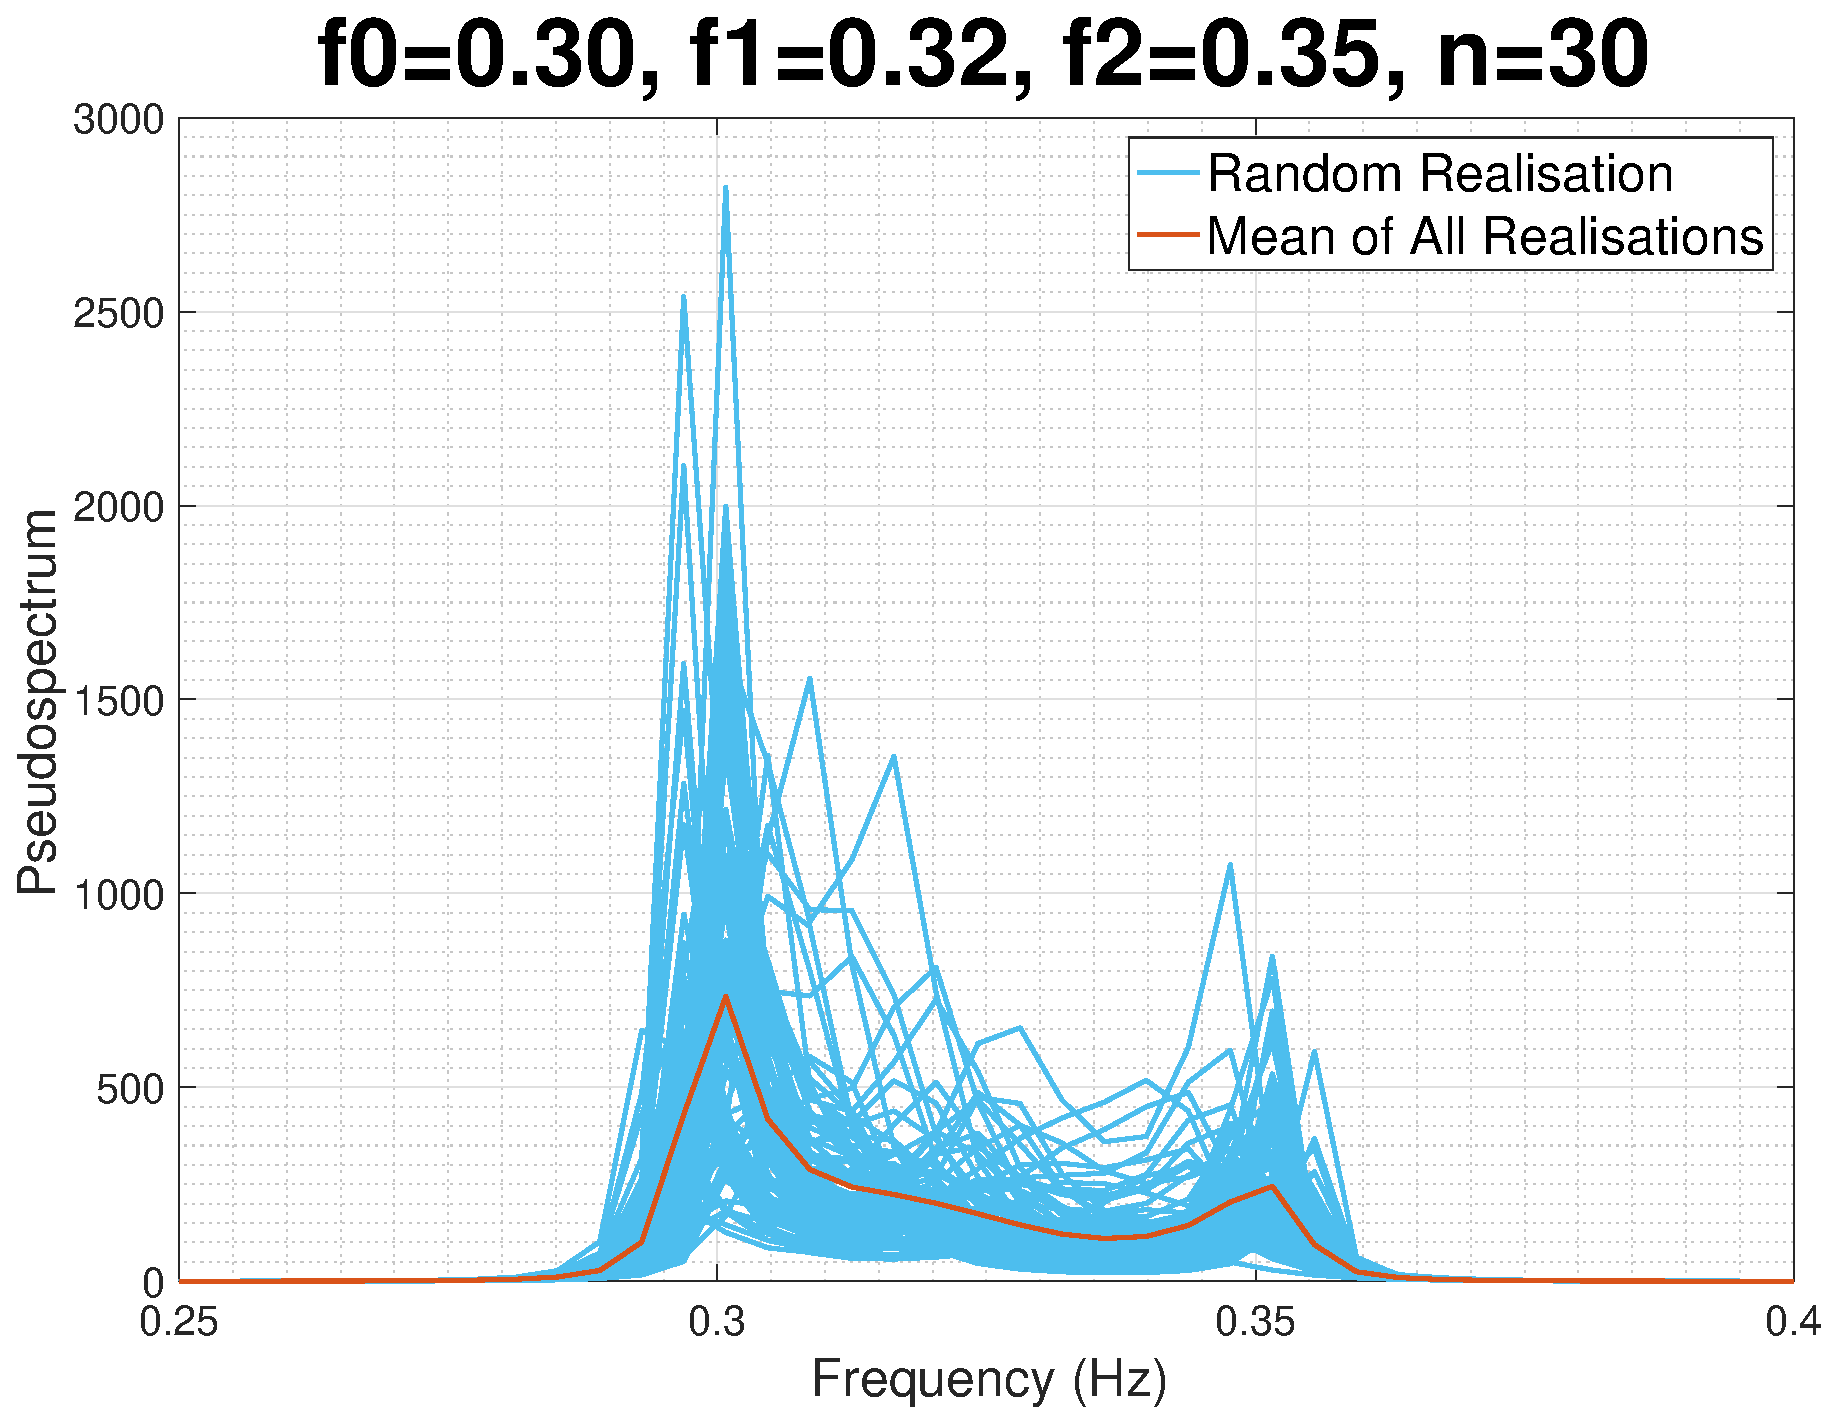
\includegraphics[width=0.32\textwidth]{part2/music_3_sinewaves_n_30_overlay}
\includegraphics[width=0.32\textwidth]{part2/music_3_sinewaves_n_70_overlay}
\caption{Detecting Sinewaves using MUSIC, and Effect of Increasing Number of Samples on the Resolution of Estimate}
\end{figure}


\begin{figure}[H]
\centering{}
\includegraphics[width=0.24\textwidth]{part2/ar_spectrum_estimate_order_4}
\includegraphics[width=0.24\textwidth]{part2/ar_spectrum_estimate_order_8}
\includegraphics[width=0.24\textwidth]{part2/ar_spectrum_estimate_order_10}
\includegraphics[width=0.24\textwidth]{part2/ar_spectrum_estimate_order_14}
\caption{Power Spectrum Estimates Using All-Pole Autoregressive Model of Orders 4, 8, 10, 14}
\end{figure}

\begin{figure}[H]
\centering{}
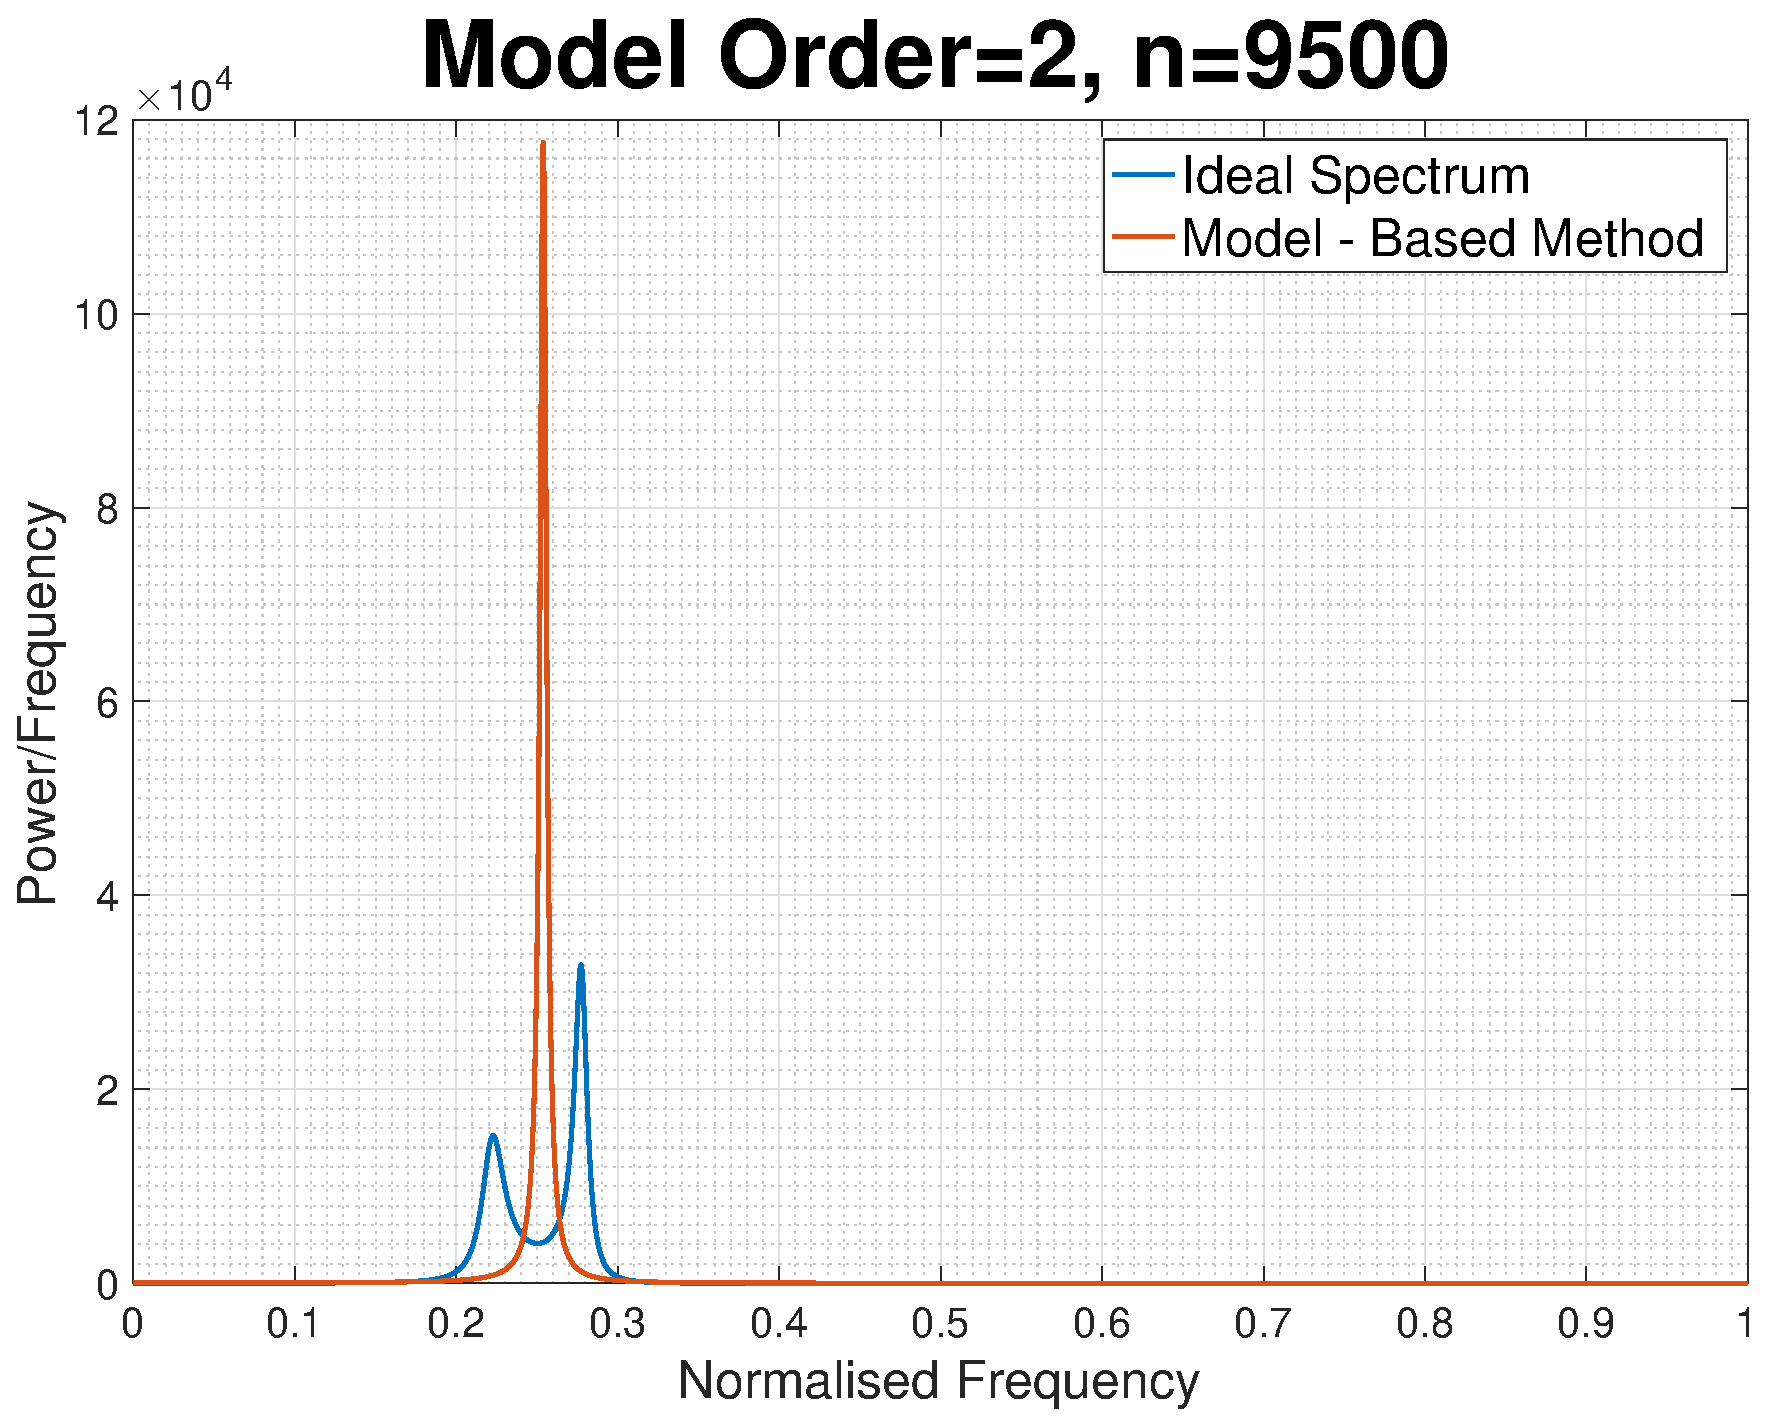
\includegraphics[width=0.32\textwidth]{part2/ar_spectrum_estimate_order_2_9500}
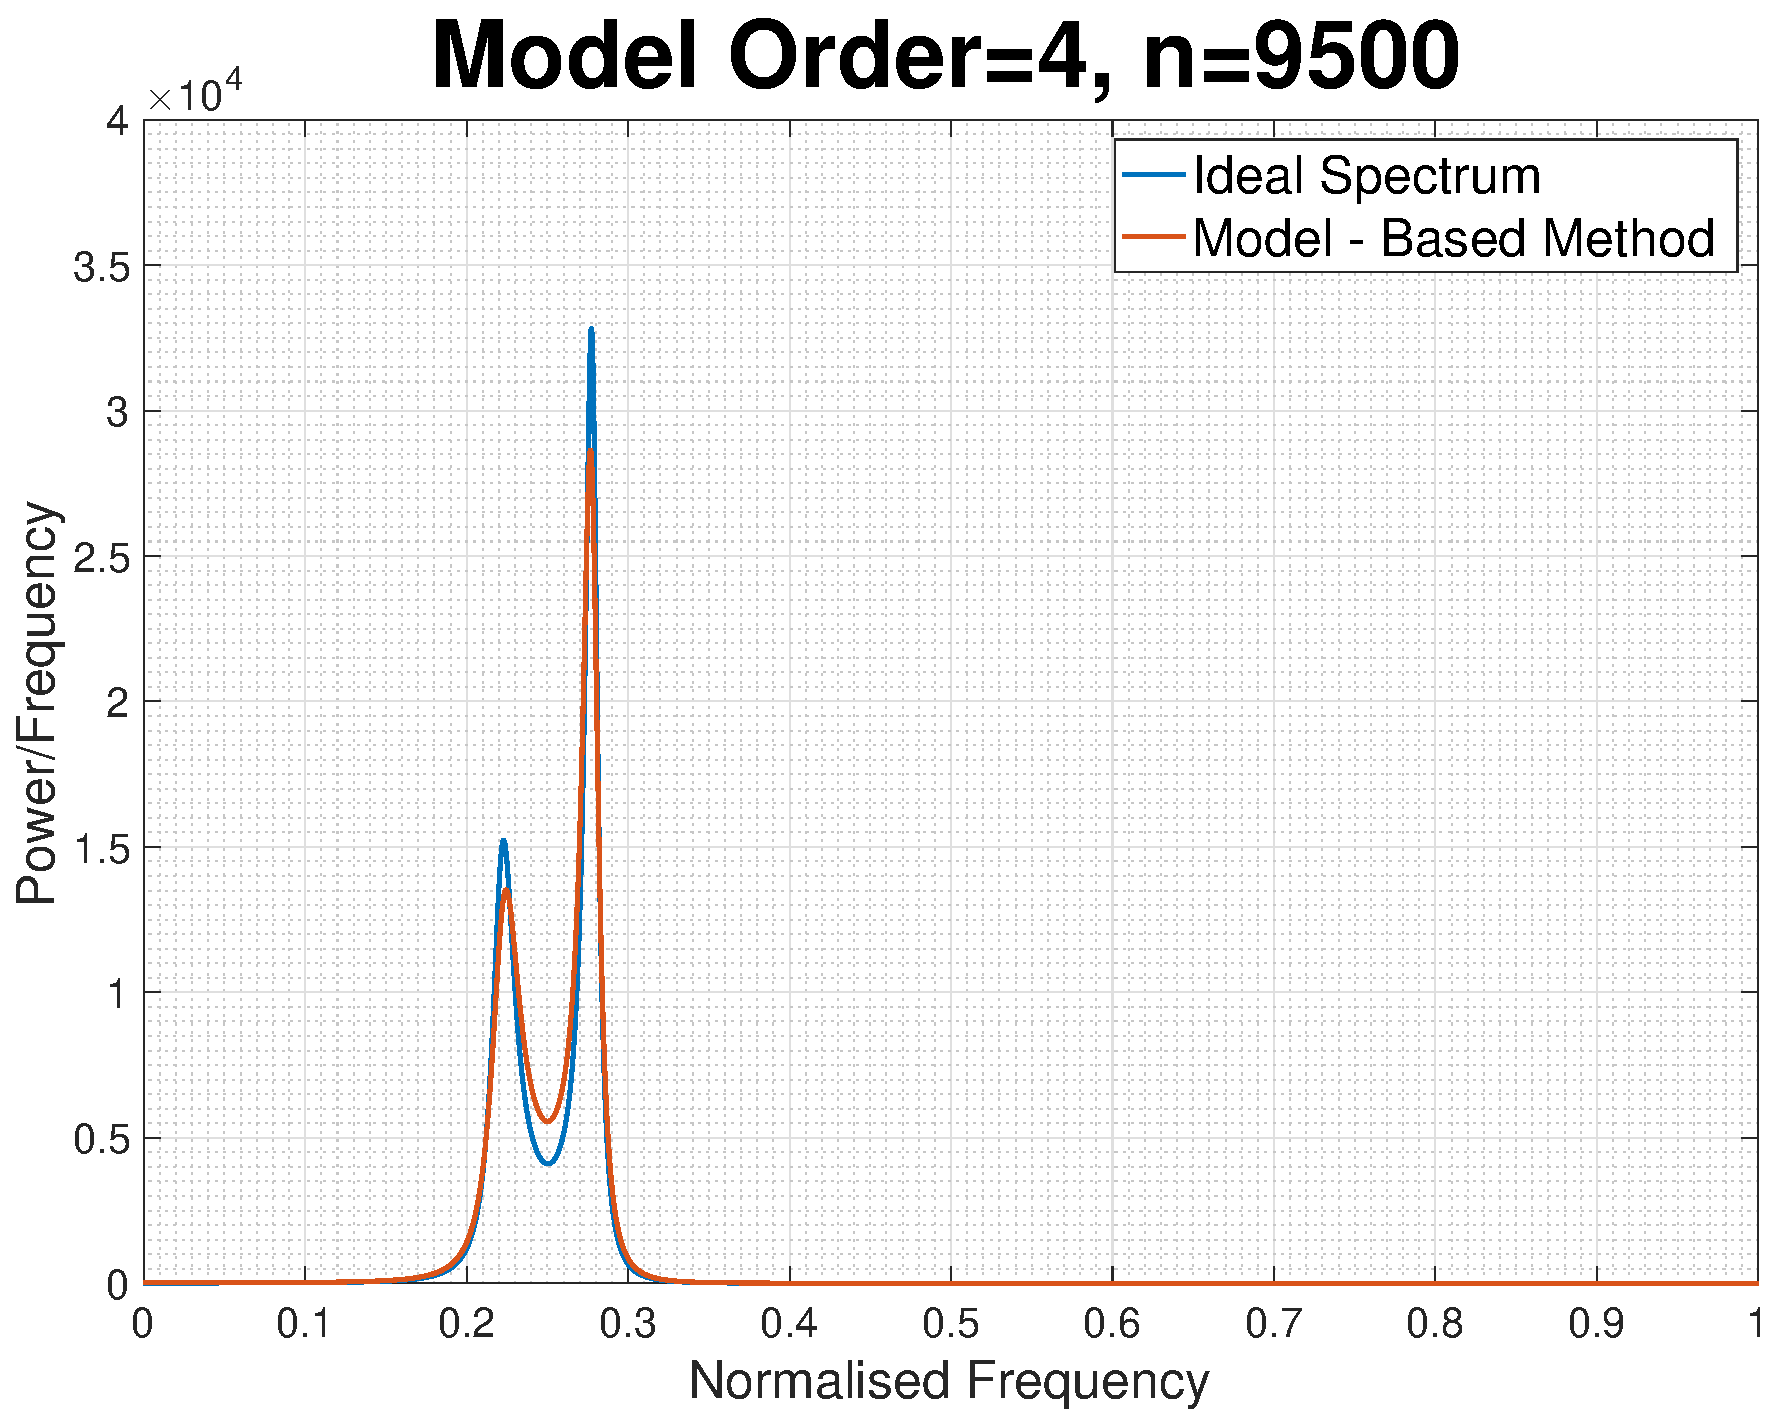
\includegraphics[width=0.32\textwidth]{part2/ar_spectrum_estimate_order_4_9500}
\includegraphics[width=0.32\textwidth]{part2/ar_spectrum_estimate_order_12_9500}
\caption{Effects of Underfitting and Overfitting Autorregressive Models}
\end{figure}

\begin{figure}[H]
\centering{}
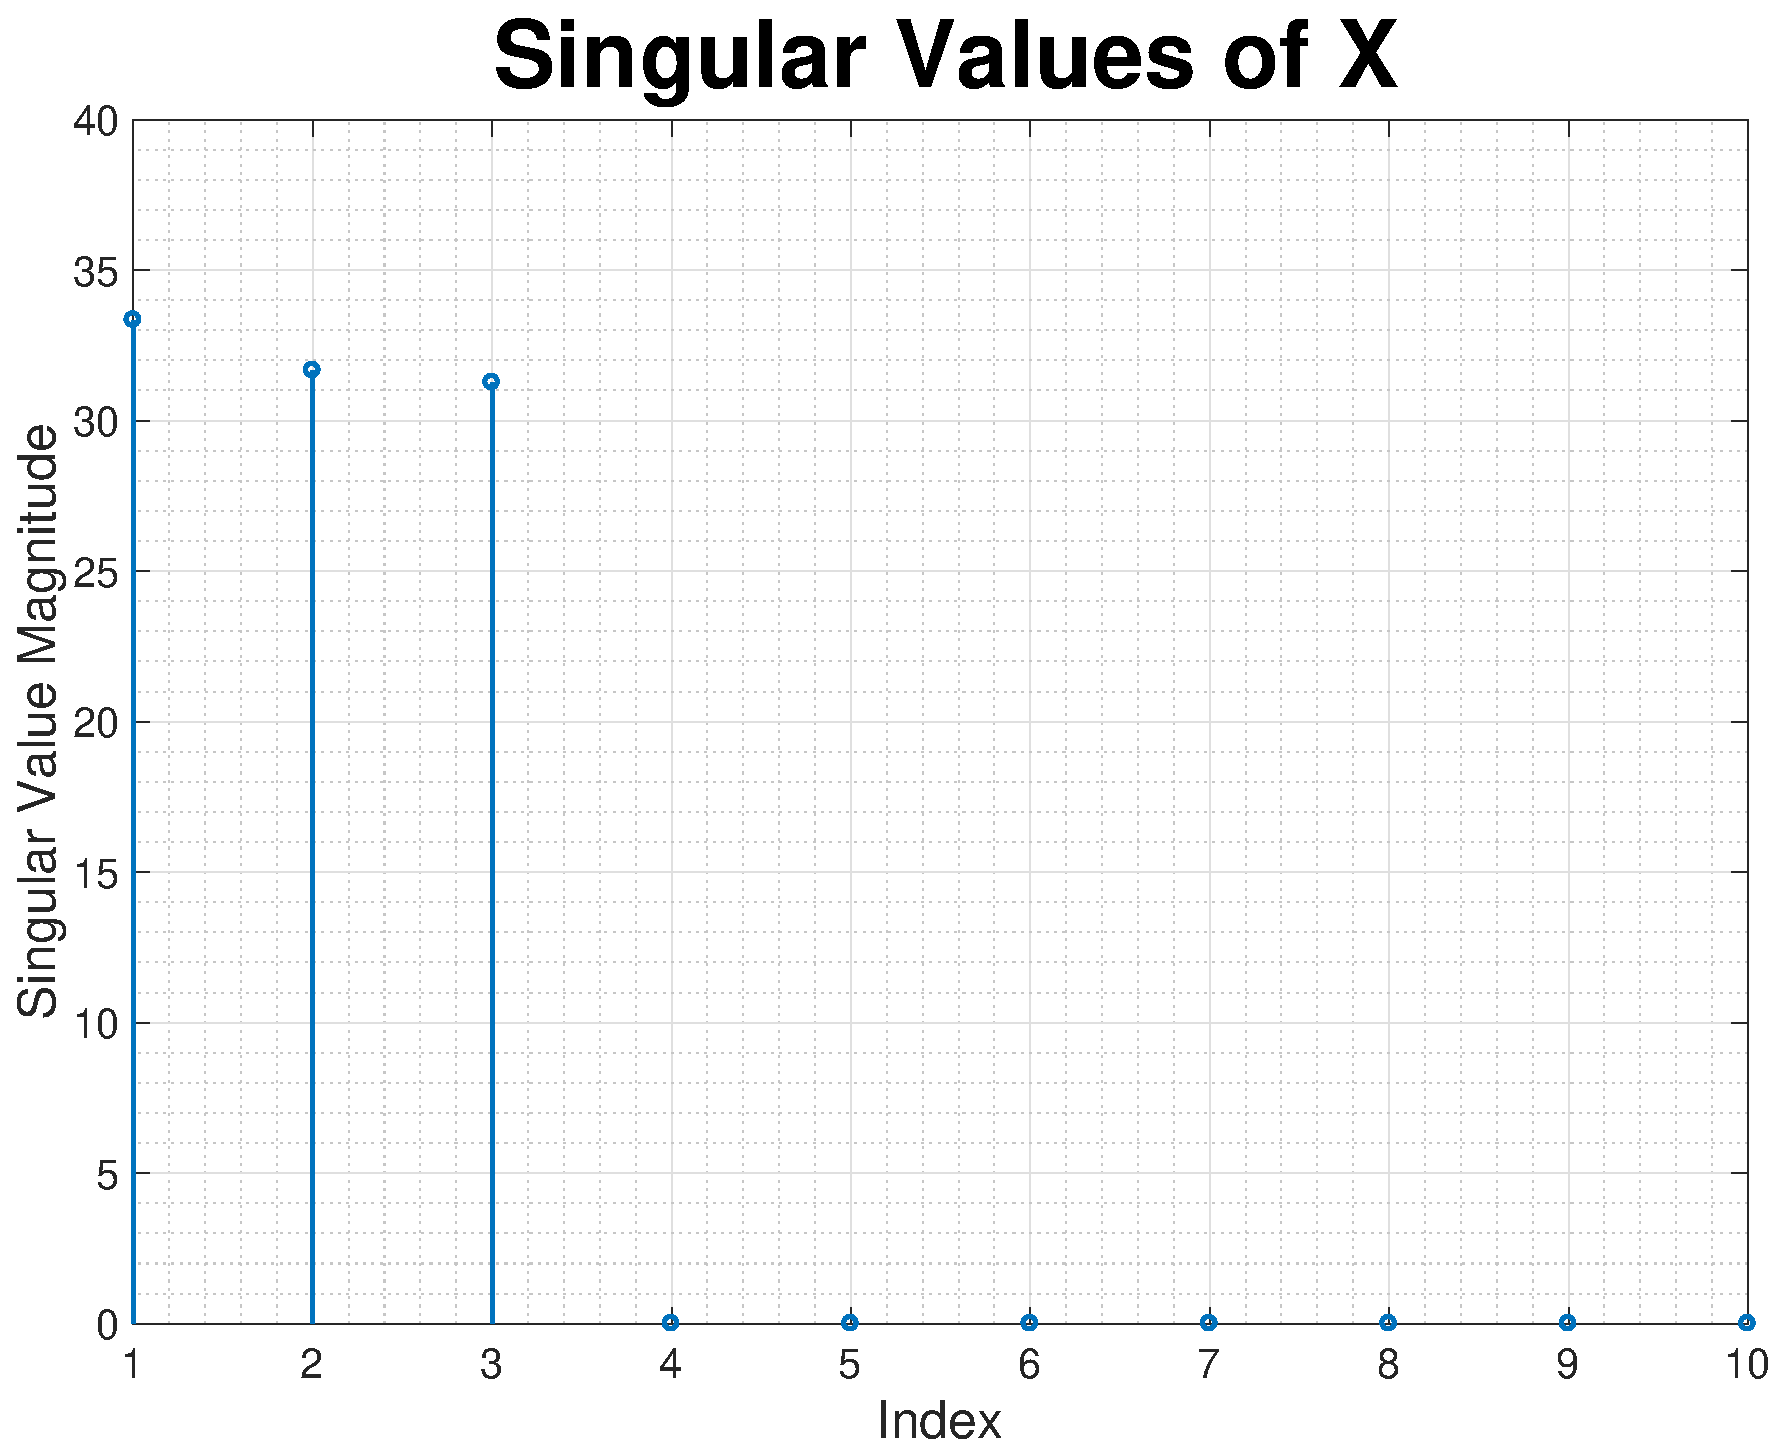
\includegraphics[width=0.32\textwidth]{part2/svd_x}
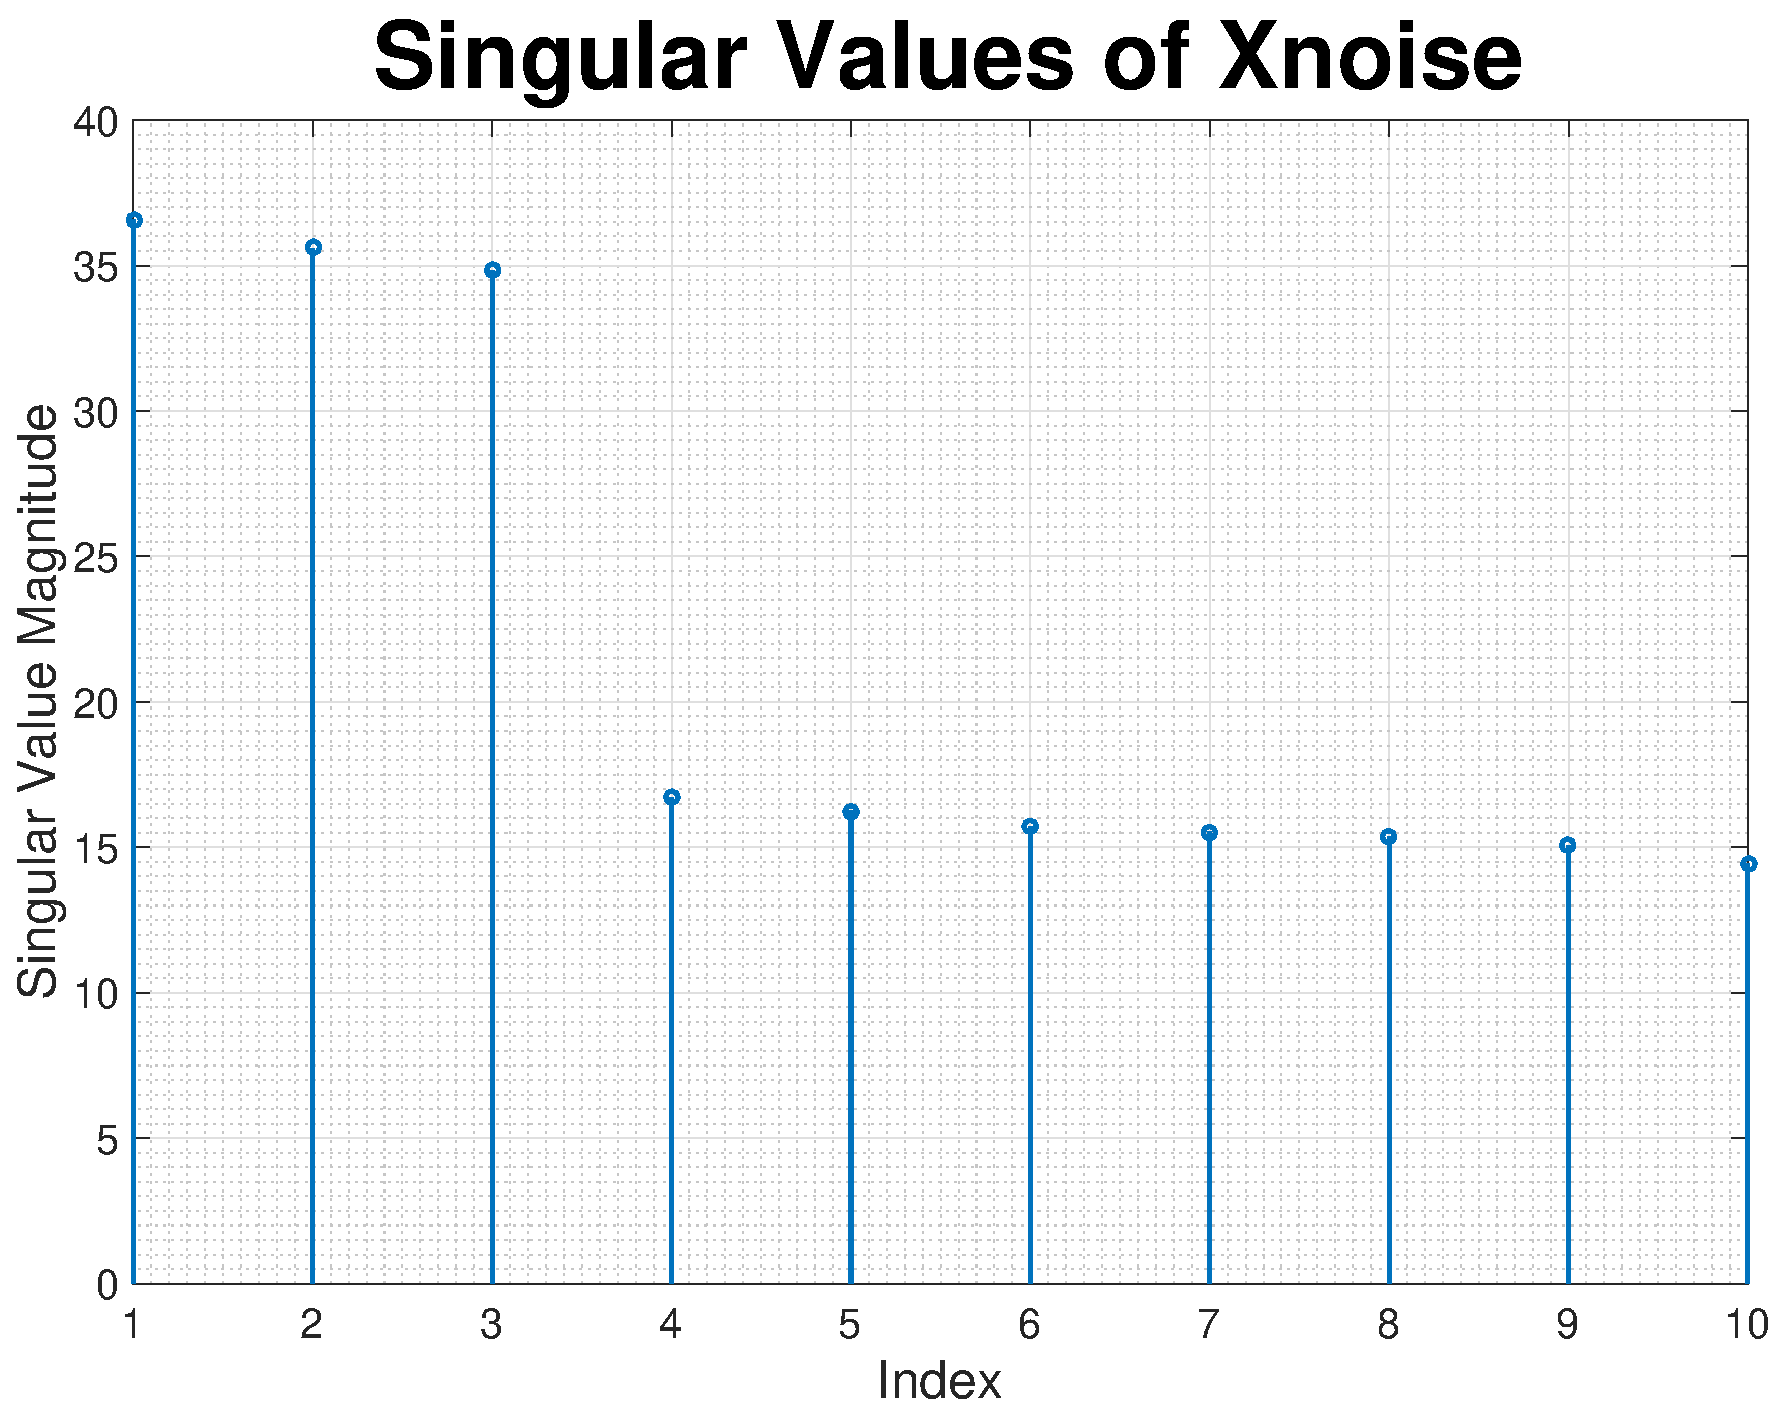
\includegraphics[width=0.32\textwidth]{part2/svd_x_noise}
\caption{Singular Values of Matrices $\textbf{X}$ and $\textbf{X}_{\text{noise}}$}
\end{figure}

\begin{figure}[H]
\centering{}
\includegraphics[width=0.32\textwidth]{part2/eeg_trial_1_standard}
\includegraphics[width=0.32\textwidth]{part2/eeg_trial_2_standard}
\includegraphics[width=0.32\textwidth]{part2/eeg_trial_3_standard}
\caption{Standard Periodograms of RRI Data obtained from Three Separate Trials}
\end{figure}

\begin{figure}[H]
\centering{}
\includegraphics[width=0.32\textwidth]{part2/eeg_trial_1_averaged}
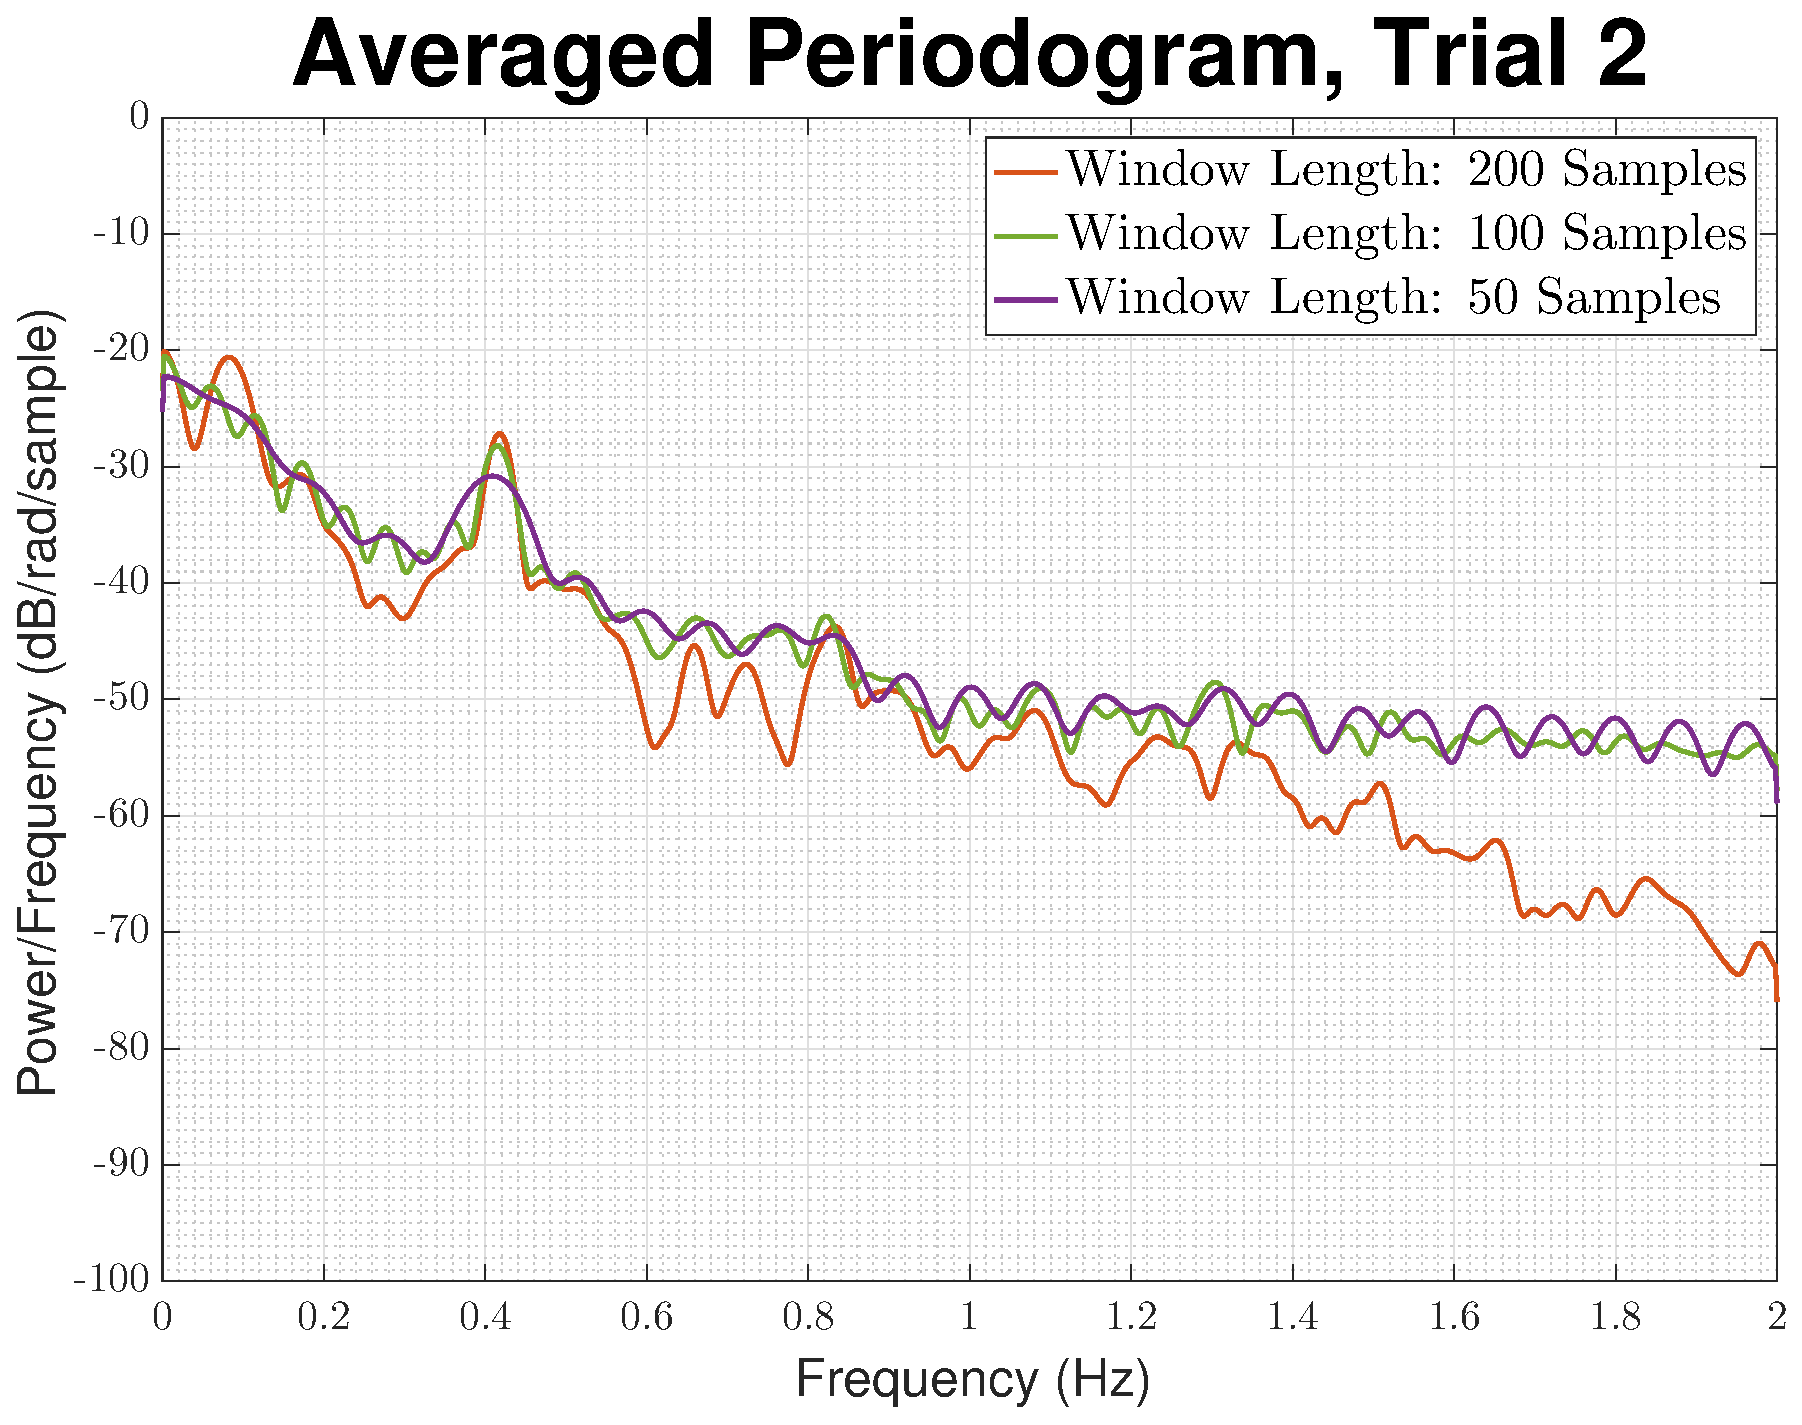
\includegraphics[width=0.32\textwidth]{part2/eeg_trial_2_averaged}
\includegraphics[width=0.32\textwidth]{part2/eeg_trial_3_averaged}
\caption{Averaged Periodograms, with Different Window Lengths, of RRI Data obtained from Three Separate Trials}
\end{figure}


\begin{figure}[H]
\centering{}
\includegraphics[width=0.32\textwidth]{part2/ar_spectrum_eeg_trial_1_order_2}
\includegraphics[width=0.32\textwidth]{part2/ar_spectrum_eeg_trial_1_order_4}
\includegraphics[width=0.32\textwidth]{part2/ar_spectrum_eeg_trial_1_order_10}
\caption{Autoregressive Spectrum Estimate for Trial 1 for Models 2, 4 and 10}
\end{figure}

\begin{figure}[H]
\centering{}
\includegraphics[width=0.32\textwidth]{part2/ar_spectrum_eeg_trial_2_order_8}
\includegraphics[width=0.32\textwidth]{part2/ar_spectrum_eeg_trial_2_order_12}
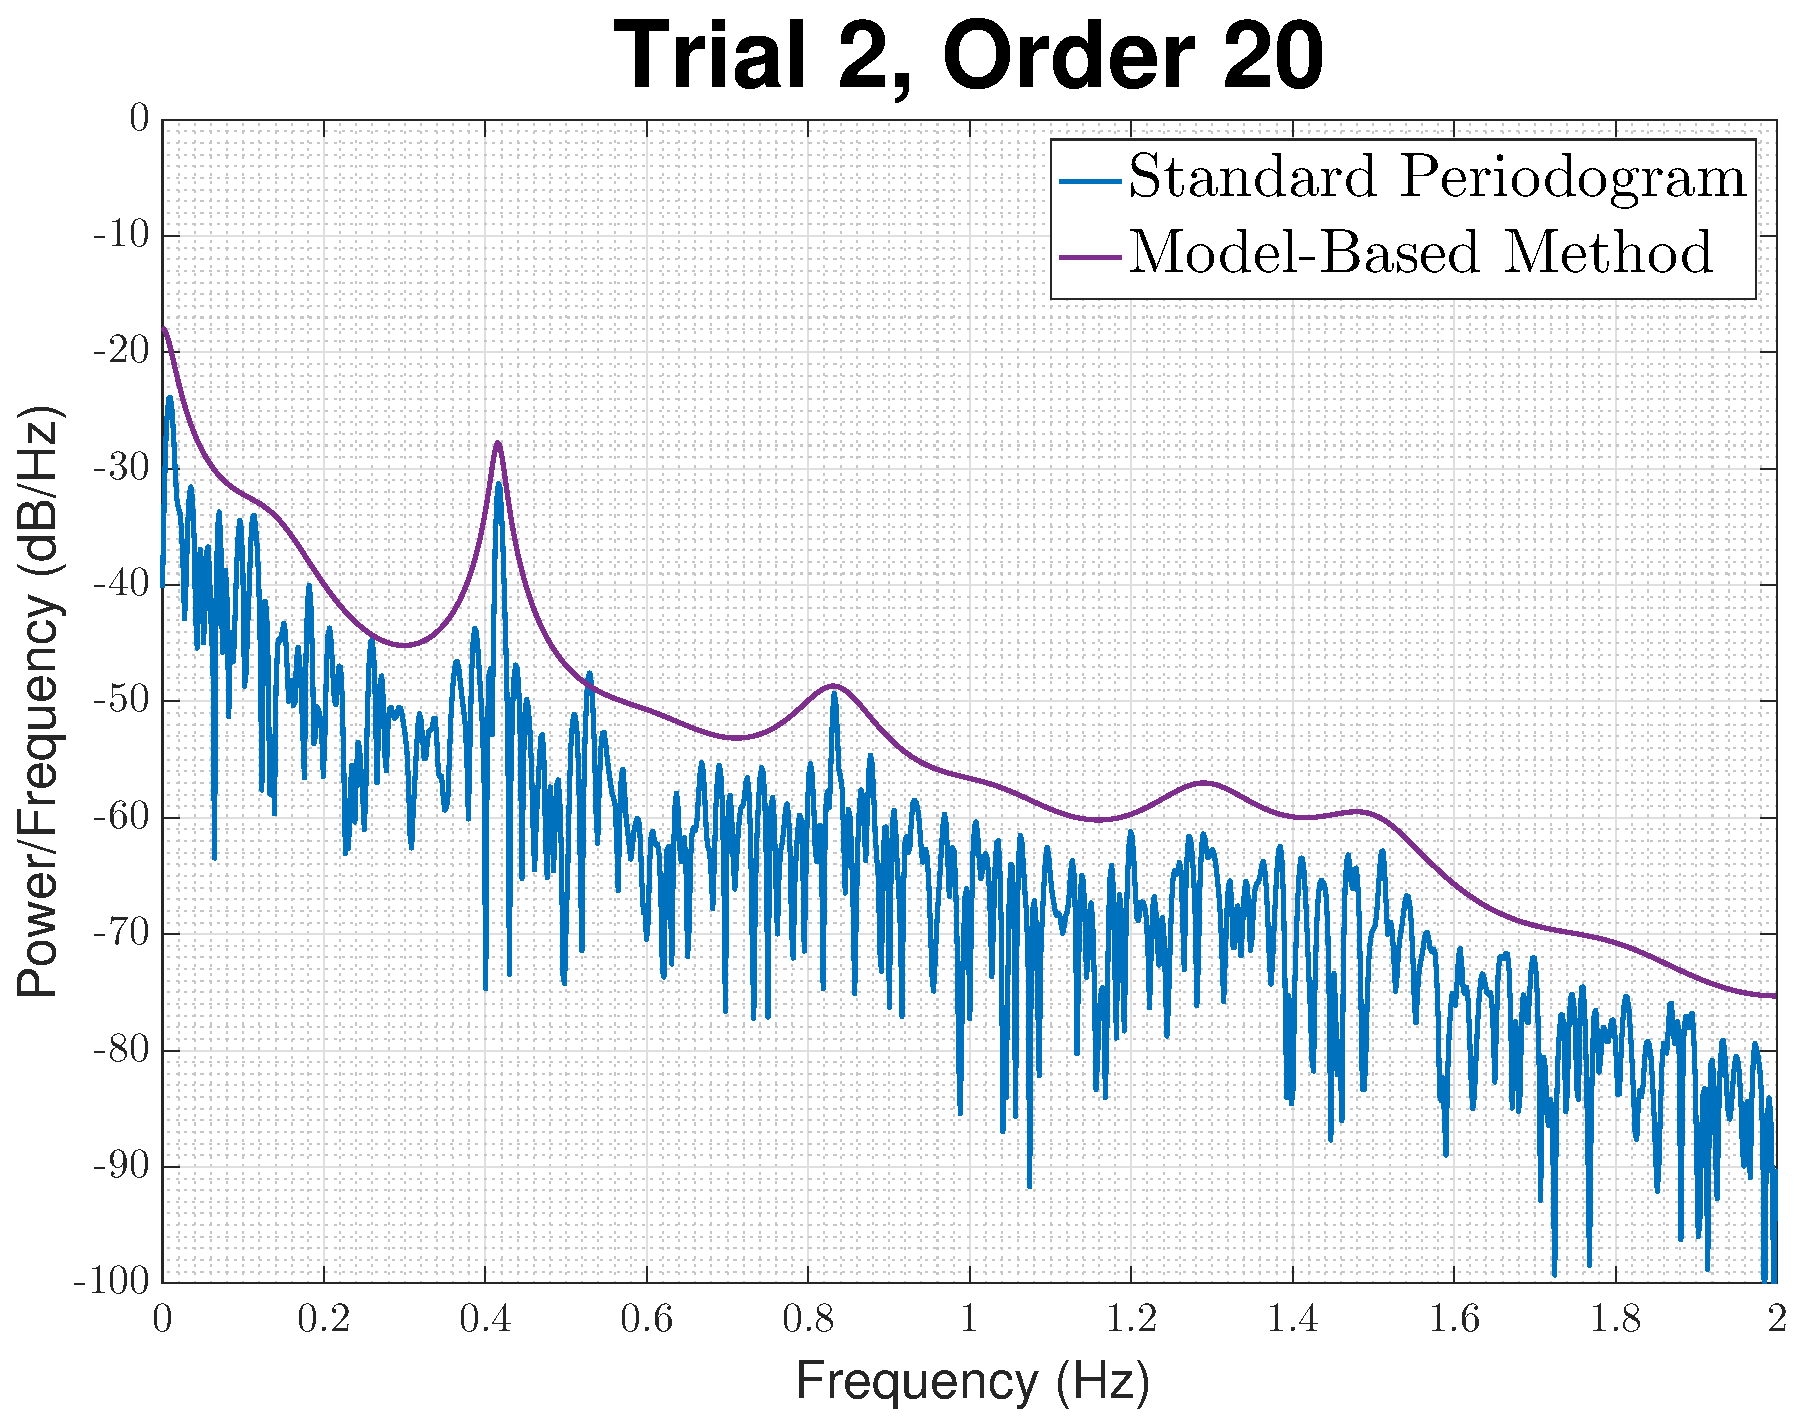
\includegraphics[width=0.32\textwidth]{part2/ar_spectrum_eeg_trial_2_order_20}
\caption{Autoregressive Spectrum Estimate for Trial 2 for Models 8, 12 and 20}
\end{figure}

\begin{figure}[H]
\centering{}
\includegraphics[width=0.32\textwidth]{part2/ar_spectrum_eeg_trial_3_order_2}
\includegraphics[width=0.32\textwidth]{part2/ar_spectrum_eeg_trial_3_order_13}
\includegraphics[width=0.32\textwidth]{part2/ar_spectrum_eeg_trial_3_order_35}
\caption{Autoregressive Spectrum Estimate for Trial 3 for Models 2, 13 and 35}
\end{figure}

